
\chapter{列王記下}
\section{北國以色列 1-8:15 }
\subsection{以色列王亞哈謝 1}
\subsubsection{亞哈謝病求問以革倫的神巴力西卜 1:1-2}
亞哈死後，摩押背叛以色列。 2 亞哈謝在撒馬利亞，一日從樓上的欄杆裡掉下來，就病了。於是差遣使者說：「你們去問以革倫的神巴力西卜，我這病能好不能好。」 3 


\subsubsection{以利亞預言亞哈謝結局 1:3-8}
但耶和華的使者對提斯比人以利亞說：「你起來，去迎著撒馬利亞王的使者，對他們說：『你們去問以革倫神巴力西卜，豈因以色列中沒有神嗎？』 4 所以耶和華如此說：『你必不下你所上的床，必定要死。』」以利亞就去了。使者回來見王，王問他們說：「你們為什麼回來呢？」 6 使者回答說：「有一個人迎著我們來，對我們說：『你們回去見差你們來的王，對他說：「耶和華如此說：你差人去問以革倫神巴力西卜，豈因以色列中沒有神嗎？所以你必不下所上的床，必定要死。」』」 7 王問他們說：「迎著你們來告訴你們這話的，是怎樣的人？」 8 回答說：「他身穿毛衣，腰束皮帶。」王說：「這必是提斯比人以利亞。」

\subsubsection{三個五十夫长與以利亞 1:9-16}
\begin{table}[H]
\centering
\begin{tabular}{p{7.5cm}|p{3.85cm}|p{4.25cm}}\hline\hline
五十夫長及隨行&以利亞/耶和華的使者&结局\\\hline\hline
於是王差遣五十夫長帶領五十人去見以利亞。他就上到以利亞那裡，以利亞正坐在山頂上。五十夫長對他說：「神人哪，王吩咐你下來！」 &以利亞回答說：「我若是神人，願火從天上降下來，燒滅你和你那五十人！」&於是有火從天上降下來，燒滅五十夫長和他那五十人。 \\\hline
王第二次差遣一個五十夫長帶領五十人去見以利亞。五十夫長對以利亞說：「神人哪，王吩咐你快快下來！」&以利亞回答說：「我若是神人，願火從天上降下來，燒滅你和你那五十人！」&於是神的火從天上降下來，燒滅五十夫長和他那五十人。 \\\hline
王第三次差遣一個五十夫長帶領五十人去。這五十夫長上去，雙膝跪在以利亞面前，哀求他說：「神人哪，願我的性命和你這五十個僕人的性命在你眼前看為寶貴！已經有火從天上降下來，燒滅前兩次來的五十夫長和他們各自帶的五十人，現在願我的性命在你眼前看為寶貴！」&耶和華的使者對以利亞說：「你同著他下去，不要怕他。」&以利亞就起來，同著他下去見王，對王說：「耶和華如此說：你差人去問以革倫神巴力西卜，豈因以色列中沒有神可以求問嗎？所以你必不下所上的床，必定要死。」\\\hline
\end{tabular}
\caption{三個五十夫长與以利亞}
\end{table}


\subsubsection{亞哈謝之死 1:17-18}
亞哈謝果然死了，正如耶和華藉以利亞所說的話。因他沒有兒子，他兄弟約蘭接續他做王，正在猶大王約沙法的兒子約蘭第二年。 18 亞哈謝其餘所行的事都寫在《以色列諸王記》上。

\subsection{先知以利亞和以利沙 2}
\subsubsection{從吉甲->伯特利->耶利哥->約旦河 2:1-8}
\begin{table}[H]
\centering
\begin{tabular}{p{3.75cm}|p{5.1cm}|p{5.1cm}|p{2.95cm}}\hline\hline
吉甲->伯特利&伯特利->耶利哥&耶利哥->約旦河&過約旦河\\\hline\hline
耶和華要用旋風接以利亞升天的時候，以利亞與以利沙從吉甲前往。以利亞對以利沙說：「耶和華差我往伯特利去，你可以在這裡等候。」以利沙說：「我指著永生的耶和華，又敢在你面前起誓：我必不離開你！」&於是二人下到伯特利。住伯特利的先知門徒出來見以利沙，對他說：「耶和華今日要接你的師傅離開你，你知道不知道？」他說：「我知道，你們不要作聲。」以利亞對以利沙說：「耶和華差遣我往耶利哥去，你可以在這裡等候。」以利沙說：「我指著永生的耶和華，又敢在你面前起誓：我必不離開你！」
&於是二人到了耶利哥。住耶利哥的先知門徒就近以利沙，對他說：「耶和華今日要接你的師傅離開你，你知道不知道？」他說：「我知道，你們不要作聲。」以利亞對以利沙說：「耶和華差遣我往約旦河去，你可以在這裡等候。」以利沙說：「我指著永生的耶和華，又敢在你面前起誓：我必不離開你！」
&於是二人一同前往。有先知門徒去了五十人，遠遠地站在他們對面，二人在約旦河邊站住。以利亞將自己的外衣捲起來，用以打水，水就左右分開，二人走乾地而過。
\\\hline
\end{tabular}
\caption{從吉甲->伯特利->耶利哥->約旦河}
\end{table}


\subsubsection{以利亞被接升天，以利沙得加倍的靈 2:9-14}
\begin{table}[H]
\centering
\begin{tabular}{p{7.cm}|p{3.85cm}|p{6.cm}}\hline\hline
以利沙求感加倍的靈&以利亞被接升天&以利沙得加倍的靈\\\hline\hline
過去之後，以利亞對以利沙說：「我未曾被接去離開你，你要我為你做什麼，只管求我。」
&\multirow{3}{4.cm}{他們正走著說話，忽有火車火馬將二人隔開，以利亞就乘旋風升天去了。以利沙看見，就呼叫說：「我父啊！我父啊！以色列的戰車馬兵啊！」}
&\multirow{3}{6.1cm}{以後不再見他了。於是以利沙把自己的衣服撕為兩片。他拾起以利亞身上掉下來的外衣，回去站在約旦河邊。他用以利亞身上掉下來的外衣打水，說：「耶和華以利亞的神在哪裡呢？」打水之後，水也左右分開，以利沙就過來了。}\\\cline{1-1}
以利沙說：「願感動你的靈加倍地感動我。」&&\\\cline{1-1}
以利亞說：「你所求的難得。雖然如此，我被接去離開你的時候，你若看見我，就必得著，不然必得不著了。」&&\\\hline
\end{tabular}
\caption{以利亞被接升天，以利沙得加倍的靈}
\end{table}


\subsubsection{耶利哥五十先知門徒尋以利亞 2:15-18}
\begin{table}[H]
\hspace*{-7mm}
\centering
\begin{tabular}{p{11.5cm}|p{7.cm}}\hline\hline
耶利哥的先知門徒&以利沙\\\hline\hline
住耶利哥的先知門徒從對面看見他就說：「感動以利亞的靈感動以利沙了。」他們就來迎接他，在他面前俯伏於地對他說：「僕人們這裡有五十個壯士，求你容他們去尋找你師傅，或者耶和華的靈將他提起來投在某山某谷。」
&以利沙說：「你們不必打發人去。」\\\hline
他們再三催促他，&他難以推辭，就說：「你們打發人去吧。」\\\hline
他們便打發五十人去，尋找了三天，也沒有找著。&以利沙仍然在耶利哥，等候他們回到他那裡，他對他們說：「我豈沒有告訴你們不必去嗎？」\\\hline
\end{tabular}
\caption{耶利哥五十先知門徒尋以利亞}
\end{table}



\subsubsection{以利沙治好耶利哥城的水 2:19-22}
\begin{table}[H]
%\hspace*{-7mm}
\centering
\begin{tabular}{p{7.cm}|p{10.cm}}\hline\hline
耶利哥城的人&以利沙\\\hline\hline
耶利哥城的人對以利沙說：「這城的地勢美好，我主看見了，只是水惡劣，土產不熟而落。」
&以利沙說：「你們拿一個新瓶來，裝鹽給我。」\\\hline
他們就拿來給他。&他出到水源，將鹽倒在水中說：「耶和華如此說：我治好了這水，從此必不再使人死，也不再使地土不生產。」於是那水治好了，直到今日，正如以利沙所說的。\\\hline
\end{tabular}
\caption{以利沙治好耶利哥城的水}
\end{table}


\subsubsection{回伯特利路上咒詛耶利哥的童子 2:23-25}
\begin{table}[H]
%\hspace*{-7mm}
\centering
\begin{tabular}{p{8.6cm}|p{9.cm}}\hline\hline
以利沙&戲笑的童子\\\hline\hline
以利沙從那裡上伯特利去。&正上去的時候，有些童子從城裡出來，戲笑他說：「禿頭的，上去吧！禿頭的，上去吧！」\\\hline
他回頭看見，就奉耶和華的名咒詛他們。&於是有兩個母熊從林中出來，撕裂他們中間四十二個童子。\\\hline
以利沙從伯特利上迦密山，又從迦密山回到撒馬利亞。&\\\hline
\end{tabular}
\caption{以利沙咒詛耶利哥的童子}
\end{table}


\begin{figure}%{.5\linewidth}
\centering
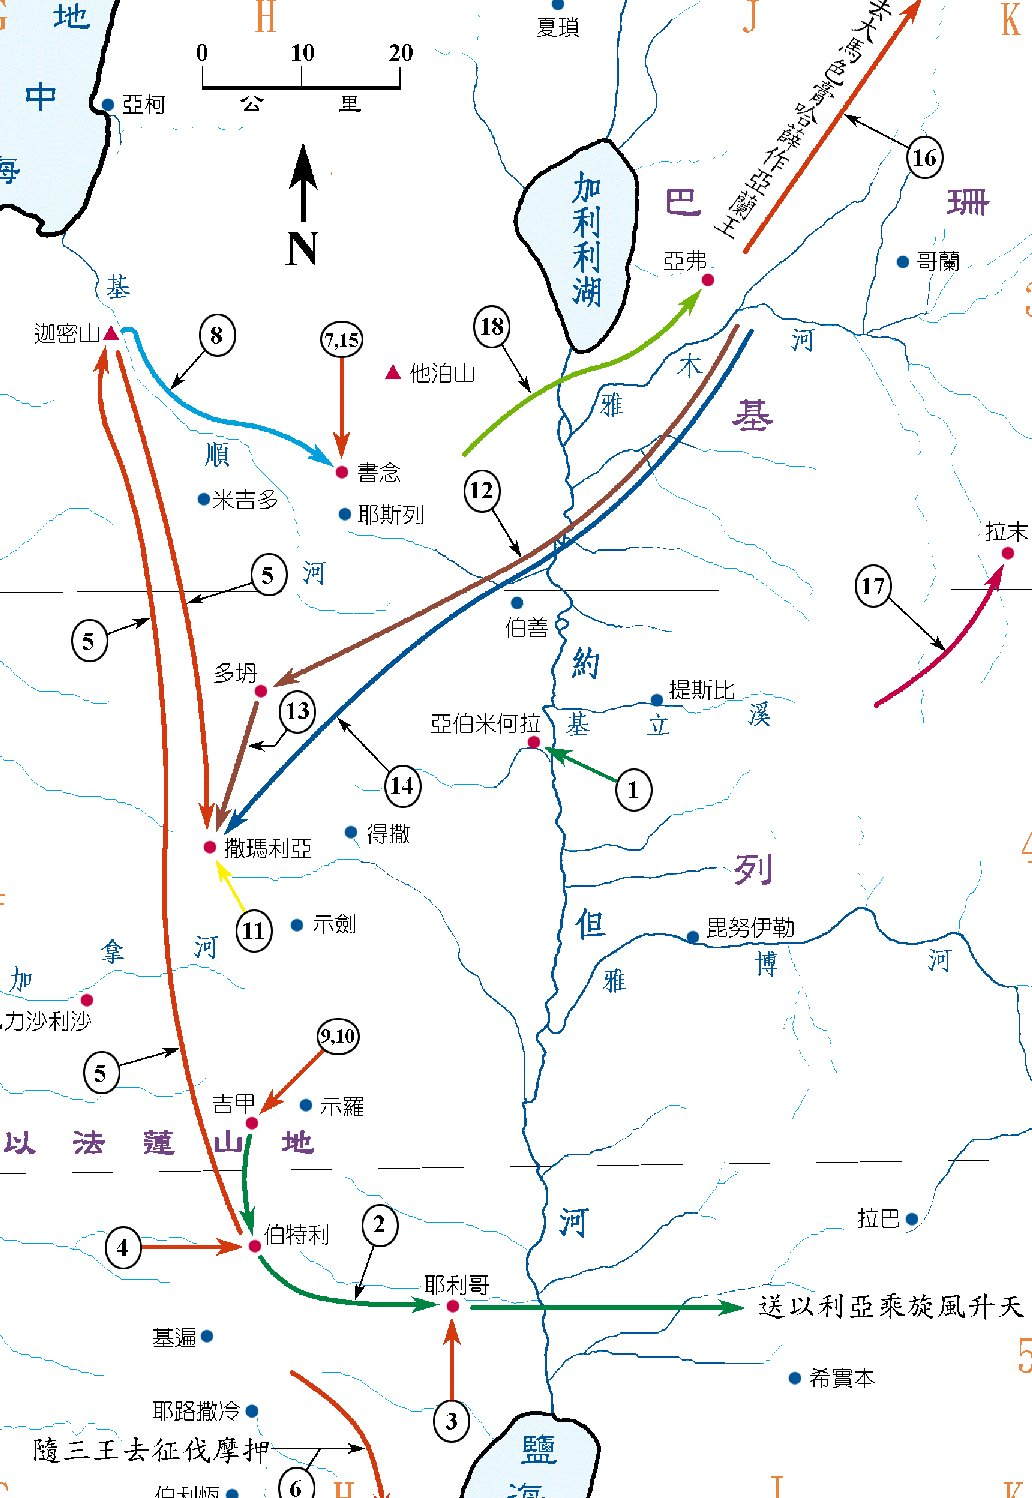
\includegraphics[width=6.25in]{BLiShiFigs/YILIYA}
\caption{以利沙的行程}
\label{fig:sub1}
\end{figure}


\newpage
\subsection{以色列王約蘭 3}
\subsubsection{約蘭做以色列王 3:1-3}
猶大王約沙法十八年，亞哈的兒子約蘭在撒馬利亞登基，做了以色列王十二年。 2 他行耶和華眼中看為惡的事，但不至像他父母所行的，因為除掉他父所造巴力的柱像。 3 然而，他貼近尼八的兒子耶羅波安使以色列人陷在罪裡的那罪，總不離開。

\subsubsection{摩押王米沙叛,邀猶大王約沙法攻打摩押 3:4-8}
摩押王米沙牧養許多羊，每年將十萬羊羔的毛和十萬公綿羊的毛給以色列王進貢。 5 亞哈死後，摩押王背叛以色列王。 6 那時約蘭王出撒馬利亞，數點以色列眾人。 7 前行的時候，差人去見猶大王約沙法，說：「摩押王背叛我，你肯同我去攻打摩押嗎？」他說：「我肯上去。你我不分彼此，我的民與你的民一樣，我的馬與你的馬一樣。」 8 約蘭說：「我們從哪條路上去呢？」回答說：「從以東曠野的路上去。」

\subsubsection{三王合攻摩押，因无水求問先知以利沙 3:9-12}
於是，以色列王和猶大王並以東王都一同去。繞行七日的路程，軍隊和所帶的牲畜沒有水喝。 10 以色列王說：「哀哉！耶和華招聚我們這三王，乃要交在摩押人的手裡！」 11 約沙法說：「這裡不是有耶和華的先知嗎？我們可以託他求問耶和華。」以色列王的一個臣子回答說：「這裡有沙法的兒子以利沙，就是從前服侍以利亞的（倒水在以利亞手上的）。」 12 約沙法說：「他必有耶和華的話。」於是以色列王和約沙法並以東王都下去見他。

\subsubsection{以利沙的預言 3:13-19}
\begin{table}[H]
\centering
\begin{tabular}{p{11.cm}|p{6.25cm}}\hline\hline
以利沙& \\\hline\hline
以利沙對以色列王說：「我與你何干？去問你父親的先知和你母親的先知吧！」&以色列王對他說：「不要這樣說，耶和華招聚我們這三王，乃要交在摩押人的手裡。」\\\hline
以利沙說：「我指著所侍奉永生的萬軍耶和華起誓，我若不看猶大王約沙法的情面，必不理你，不顧你。現在你們給我找一個彈琴的來。」&彈琴的時候，耶和華的靈（手）就降在以利沙身上。\\\hline
他便說：「耶和華如此說：你們要在這谷中滿處挖溝。因為耶和華如此說：你們雖不見風，不見雨，這谷必滿了水，使你們和牲畜有水喝。在耶和華眼中這還算為小事，他也必將摩押人交在你們手中。你們必攻破一切堅城美邑，砍伐各種佳樹，塞住一切水泉，用石頭糟蹋一切美田。」&次日早晨，約在獻祭的時候，有水從以東而來，遍地就滿了水。\\\hline
\end{tabular}
\caption{三王戰敗摩押}
\end{table}
 

\subsubsection{摩押人敗遁 3:20-27}
\begin{wrapfigure}{r}{.5\linewidth}
\vspace{-6mm}
\centering
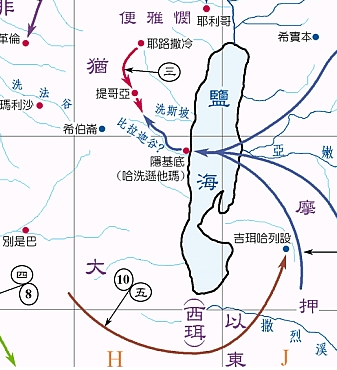
\includegraphics[width=3in]{BLiShiFigs/moya}
\caption{三王戰敗摩押}
\label{fig:sub1}
\end{wrapfigure}
摩押眾人聽見這三王上來要與他們爭戰，凡能頂盔貫甲的，無論老少，盡都聚集站在邊界上。 22 次日早晨，日光照在水上，摩押人起來，看見對面水紅如血，就說： 23 「這是血啊！必是三王互相擊殺，俱都滅亡。摩押人哪，我們現在去搶奪財物吧！」 24 摩押人到了以色列營，以色列人就起來攻打他們，以致他們在以色列人面前逃跑。以色列人往前追殺摩押人，直殺入摩押的境內， 25 拆毀摩押的城邑，各人拋石填滿一切美田，塞住一切水泉，砍伐各種佳樹，只剩下吉珥哈列設的石牆，甩石的兵在四圍攻打那城。 26 摩押王見陣勢甚大，難以對敵，就率領七百拿刀的兵，要衝過陣去到以東王那裡，卻是不能。 27 便將那應當接續他做王的長子，在城上獻為燔祭。以色列人遭遇耶和華的大怒（招人痛恨），於是三王離開摩押王，各回本國去了。

\subsection{先知以利沙的服事 4-8:15}
\subsubsection{幫助先知遺孀還債 4:1-7}
\begin{table}[H]
\centering
\begin{tabular}{p{10.cm}|p{7.25cm}}\hline\hline
先知門徒的妻&以利沙\\\hline
有一個先知門徒的妻哀求以利沙說：「你僕人我丈夫死了，他敬畏耶和華是你所知道的。現在有債主來，要取我兩個兒子做奴僕。」
& 以利沙問她說：「我可以為你做什麼呢？你告訴我，你家裡有什麼？」\\\hline
她說：「婢女家中除了一瓶油之外，沒有什麼。」&以利沙說：「你去，向你眾鄰舍借空器皿，不要少借。回到家裡，關上門，你和你兒子在裡面將油倒在所有的器皿裡，倒滿了的放在一邊。」\\\hline
於是婦人離開以利沙去了，關上門，自己和兒子在裡面，兒子把器皿拿來，她就倒油。器皿都滿了，她對兒子說：「再給我拿器皿來。」兒子說：「再沒有器皿了。」油就止住了。婦人去告訴神人，&神人說：「你去賣油還債，所剩的，你和你兒子可以靠著度日。」\\\hline
\end{tabular}
\caption{幫助先知遺孀還債}
\end{table}


\subsubsection{書念婦接待以利沙得子 4:8-17}
\begin{table}[H]
\centering
\begin{tabular}{p{5.5cm}|p{5.75cm}|p{6.cm}}\hline\hline
書念婦接待以利沙&以利沙问婦人所求&婦人得子\\\hline
一日，以利沙走到書念，在那裡有一個大戶的婦人強留他吃飯。此後以利沙每從那裡經過，就進去吃飯。婦人對丈夫說：「我看出那常從我們這裡經過的是聖潔的神人。我們可以為他在牆上蓋一間小樓，在其中安放床榻、桌子、椅子、燈臺，他來到我們這裡，就可以住在其間。」
&一日以利沙來到那裡，就進了那樓躺臥。以利沙吩咐僕人基哈西說：「你叫這書念婦人來。」他就把婦人叫了來，婦人站在以利沙面前。以利沙吩咐僕人說：「你對她說：『你既為我們費了許多心思，可以為你做什麼呢？你向王或元帥有所求的沒有？』」她回答說：「我在我本鄉安居無事。」
&以利沙對僕人說：「究竟當為她做什麼呢？」基哈西說：「她沒有兒子，她丈夫也老了。」以利沙說：「再叫她來。」於是叫了她來，她就站在門口。以利沙說：「明年到這時候，你必抱一個兒子。」她說：「神人，我主啊，不要那樣欺哄婢女！」婦人果然懷孕，到了那時候，生了一個兒子，正如以利沙所說的。\\\hline
\end{tabular}
\caption{書念婦接待以利沙得子}
\end{table}

\subsubsection{幫助書念婦人兒子死里复活 4:18-37}
\begin{table}[H]
\centering
\begin{tabular}{p{5.15cm}|p{5.5cm}|p{6.cm}}\hline\hline
孩子因頭疾而死&婦人跪求神人&兒子死里复活\\\hline
孩子漸漸長大，一日到他父親和收割的人那裡。他對父親說：「我的頭啊！我的頭啊！」他父親對僕人說：「把他抱到他母親那裡。」僕人抱去，交給他母親，孩子坐在母親的膝上，到晌午就死了。他母親抱他上了樓，將他放在神人的床上，關上門出來，呼叫她丈夫說：「你叫一個僕人，給我牽一匹驢來，我要快快地去見神人，就回來。」丈夫說：「今日不是月朔，也不是安息日，你為何要去見他呢？」婦人說：「平安無事。」於是備上驢，對僕人說：「你快快趕著走，我若不吩咐你，就不要遲慢。」婦人就往迦密山去見神人。
&神人遠遠地看見她，對僕人基哈西說：「看哪，書念的婦人來了。你跑去迎接她，問她說：『你平安嗎？你丈夫平安嗎？孩子平安嗎？』」她說：「平安。」婦人上了山，到神人那裡，就抱住神人的腳。基哈西前來要推開她，神人說：「由她吧！因為她心裡愁苦。耶和華向我隱瞞，沒有指示我。」婦人說：「我何嘗向我主求過兒子呢？我豈沒有說過，不要欺哄我嗎？」以利沙吩咐基哈西說：「你束上腰，手拿我的杖前去。若遇見人，不要向他問安，人若向你問安，也不要回答。要把我的杖放在孩子臉上。」孩子的母親說：「我指著永生的耶和華，又敢在你面前起誓：我必不離開你！」
&於是以利沙起身，隨著她去了。基哈西先去，把杖放在孩子臉上，卻沒有聲音，也沒有動靜。基哈西就迎著以利沙回來，告訴他說：「孩子還沒有醒過來。」以利沙來到，進了屋子，看見孩子死了，放在自己的床上。他就關上門，只有自己和孩子在裡面，他便祈禱耶和華。上床伏在孩子身上，口對口，眼對眼，手對手。既伏在孩子身上，孩子的身體就漸漸溫和了。然後他下來，在屋裡來往走了一趟，又上去伏在孩子身上。孩子打了七個噴嚏，就睜開眼睛了。以利沙叫基哈西說：「你叫這書念婦人來。」於是叫了她來。以利沙說：「將你兒子抱起來。」婦人就進來，在以利沙腳前俯伏於地，抱起她兒子出去了。\\\hline
\end{tabular}
\caption{書念婦接待以利沙得子}
\end{table}


\subsubsection{在吉甲解除野瓜湯的毒 4:38-41}
\begin{table}[H]
\centering
\begin{tabular}{p{5.5cm}|p{11.25cm}}\hline\hline
以利沙&先知門徒\\\hline
以利沙又來到吉甲，那地正有饑荒。&先知門徒坐在他面前，\\\hline
他吩咐僕人說：「你將大鍋放在火上，給先知門徒熬湯。」&有一個人去到田野掐菜，遇見一棵野瓜藤，就摘了一兜野瓜回來，切了擱在熬湯的鍋中，因為他們不知道是什麼東西。倒出來給眾人吃，吃的時候，都喊叫說：「神人哪，鍋中有致死的毒物！」所以眾人不能吃了。\\\hline
以利沙說：「拿點麵來。」就把麵撒在鍋中，說：「倒出來給眾人吃吧。」&鍋中就沒有毒了。\\\hline
\end{tabular}
\caption{在吉甲解除野瓜湯的毒}
\end{table}
 

\subsubsection{用二十個大麥餅餵飽一百人 4:42-44}
\begin{table}[H]
\centering
\begin{tabular}{p{4.5cm}|p{6.25cm}|p{6.cm}}\hline\hline
二十個餅&以利沙&僕人\\\hline
\multirow{2}{4.6cm}{有一個人從巴力沙利沙來，帶著初熟大麥做的餅二十個並新穗子，裝在口袋裡送給神人。}&神人說：「把這些給眾人吃。」&僕人說：「這一點豈可擺給一百人吃呢？」\\\cline{2-3}
&以利沙說：「你只管給眾人吃吧，因為耶和華如此說：『眾人必吃了，還剩下。』」&僕人就擺在眾人面前。他們吃了，果然還剩下，正如耶和華所說的。\\\hline
\end{tabular}
\caption{用二十個大麥餅餵飽一百人}
\end{table}


\subsubsection{醫治乃曼的大麻風 5}
\subsubsubsection{乃縵患大痲瘋，使女荐其求治於先知 5:1-6}
\begin{table}[H]
\centering
\begin{tabular}{p{3.75cm}|p{5.cm}|p{8.25cm}}\hline\hline
乃縵患大痲瘋&以色列使女荐其求先知&亞蘭王准乃曼，达信於以色列王\\\hline
亞蘭王的元帥乃縵在他主人面前為尊為大，因耶和華曾藉他使亞蘭人得勝。他又是大能的勇士，只是長了大痲瘋。
&先前亞蘭人成群地出去，從以色列國擄了一個小女子，這女子就服侍乃縵的妻。她對主母說：「巴不得我主人去見撒馬利亞的先知，必能治好他的大痲瘋。」 
&乃縵進去，告訴他主人說：「以色列國的女子如此如此說。」亞蘭王說：「你可以去，我也達信於以色列王。」於是乃縵帶銀子十他連得、金子六千舍客勒、衣裳十套，就去了。且帶信給以色列王，信上說：「我打發臣僕乃縵去見你，你接到這信，就要治好他的大痲瘋。」\\\hline
\end{tabular}
\caption{乃縵患大痲瘋，使女荐其求治於先知}
\end{table}


\subsubsubsection{以色列王看信撕衣，以利沙接待乃縵 5:7-14}
\begin{table}[H]
\centering
\begin{tabular}{p{8.25cm}|p{8.cm}}\hline\hline
以色列王看信撕衣&以利沙接待乃縵\\\hline
以色列王看了信就撕裂衣服，說：「我豈是神，能使人死使人活呢？這人竟打發人來，叫我治好他的大痲瘋！你們看一看，這人何以尋隙攻擊我呢？」
&神人以利沙聽見以色列王撕裂衣服，就打發人去見王，說：「你為什麼撕了衣服呢？可使那人到我這裡來，他就知道以色列中有先知了。」\\\hline
\end{tabular}
\caption{乃縵患大痲瘋，使女荐其求治於先知}
\end{table}

\subsubsubsection{浴於約旦河得潔 5:7-14}
\begin{table}[H]
\centering
\begin{tabular}{p{8.5cm}|p{5.cm}|p{4.0cm}}\hline\hline
乃縵&以利沙&僕人\\\hline
於是乃縵帶著車馬到了以利沙的家，站在門前。
&以利沙打發一個使者對乃縵說：「你去在約旦河中沐浴七回，你的肉就必復原，而得潔淨。」&\\\hline
乃縵卻發怒走了說"我想他必定出來見我，站著求告耶和華他神的名，在患處以上搖手，治好這大痲瘋。大馬士革的河亞罷拿和法珥法豈不比以色列的一切水更好嗎?我在那裡沐浴不得潔淨嗎"於是氣憤憤地轉身去了。&&他的僕人進前來對他說"我父啊，先知若吩咐你做一件大事你豈不做嗎?何況說你去沐浴而得潔淨呢"\\\hline
於是乃縵下去，照著神人的話，在約旦河裡沐浴七回。他的肉復原，好像小孩子的肉，他就潔淨了。&&\\\hline
\end{tabular}
\caption{浴於約旦河得潔}
\end{table}


\subsubsubsection{乃縵饋物以利沙不受 5:15-19}
\begin{table}[H]
\centering
\begin{tabular}{p{12.cm}|p{5.cm}}\hline\hline
乃縵&以利沙\\\hline
乃縵帶著一切跟隨他的人回到神人那裡，站在他面前，說：「如今我知道，除了以色列之外，普天下沒有神。現在求你收點僕人的禮物。」
&以利沙說：「我指著所侍奉永生的耶和華起誓，我必不受。」\\\hline
乃縵再三地求他，他卻不受。乃縵說：「你若不肯受，請將兩騾子馱的土賜給僕人。從今以後，僕人必不再將燔祭或平安祭獻於別神，只獻給耶和華。唯有一件事，願耶和華饒恕你僕人：我主人進臨門廟叩拜的時候，我用手攙他在臨門廟，我也屈身。我在臨門廟屈身的這事，願耶和華饒恕我！」&以利沙對他說：「你可以平平安安地回去。」\\\hline
\end{tabular}
\caption{乃縵饋物以利沙不受}
\end{table}


\subsubsubsection{基哈西诓哄乃縵得其財 5:20-24}
\begin{table}[H]
\centering
\begin{tabular}{p{7.cm}|p{10.5cm}}\hline\hline
乃縵&基哈西\\\hline
乃縵就離開他去了，走了不遠。&神人以利沙的僕人基哈西心裡說：「我主人不願從這亞蘭人乃縵手裡受他帶來的禮物，我指著永生的耶和華起誓，我必跑去追上他，向他要些。」於是基哈西追趕乃縵。\\\hline
乃縵看見有人追趕，就急忙下車迎著他，說：「都平安嗎？」&說：「都平安。我主人打發我來說：『剛才有兩個少年人，是先知門徒，從以法蓮山地來見我，請你賜他們一他連得銀子、兩套衣裳。』」\\\hline
乃縵說：「請受二他連得。」再三地請受，便將二他連得銀子裝在兩個口袋裡，又將兩套衣裳交給兩個僕人，他們就在基哈西前頭抬著走。&到了山岡，基哈西從他們手中接過來，放在屋裡，打發他們回去。\\\hline
\end{tabular}
\caption{基哈西诓哄乃縵得其財}
\end{table}


\subsubsubsection{基哈西得財致患大痲瘋 5:25-27}
\begin{table}[H]
\centering
\begin{tabular}{p{8.cm}|p{9.5cm}}\hline\hline
基哈西&以利沙\\\hline
基哈西進去，站在他主人面前。&以利沙問他說：「基哈西，你從哪裡來？」\\\hline
回答說：「僕人沒有往哪裡去。」 &以利沙對他說：「那人下車轉回迎你的時候，我的心豈沒有去呢？這豈是受銀子、衣裳，買橄欖園、葡萄園、牛羊、僕婢的時候呢？因此，乃縵的大痲瘋必沾染你和你的後裔，直到永遠。」\\\hline
基哈西從以利沙面前退出去，就長了大痲瘋，像雪那樣白。&\\\hline
\end{tabular}
\caption{基哈西得財致患大痲瘋}
\end{table}


\subsubsection{在約旦河找到沉入水底的斧子 6:1-7}
\begin{table}[H]
\centering
\begin{tabular}{p{10.cm}|p{7.cm}}\hline\hline
基哈西&以利沙\\\hline
先知門徒對以利沙說：「看哪，我們同你所住的地方過於窄小。求你容我們往約旦河去，各人從那裡取一根木料建造房屋居住。」&他說：「你們去吧。」\\\hline
有一人說：「求你與僕人同去。」 &回答說：「我可以去。」於是以利沙與他們同去。\\\hline
到了約旦河，就砍伐樹木。有一人砍樹的時候，斧頭掉在水裡，他就呼叫說：「哀哉！我主啊，這斧子是借的。」&神人問說：「掉在哪裡了？」\\\hline
他將那地方指給以利沙看。&以利沙砍了一根木頭，拋在水裡，斧頭就漂上來了。以利沙說：「拿起來吧。」\\\hline
那人就伸手拿起來了。&\\\hline
\end{tabular}
\caption{基哈西得財致患大痲瘋}
\end{table}


\subsubsection{多次警戒以色列王防備亞蘭人的暗殺 6:8-10}
亞蘭王與以色列人爭戰，和他的臣僕商議說：「我要在某處某處安營。」 9 神人打發人去見以色列王，說：「你要謹慎，不要從某處經過，因為亞蘭人從那裡下來了。」 10 以色列王差人去窺探神人所告訴、所警戒他去的地方，就防備未受其害，不止一兩次。

\subsubsection{以利沙被亞蘭人困於多坍，开其僕眼見火車火馬 6:11-17}
\begin{tabular}{p{4.cm}|p{4.25cm}}\hline
\multicolumn{2}{c}{亞蘭人困以利沙於多坍}\\\hline
亞蘭王因這事心裡驚疑，召了臣僕來，對他們說：「我們這裡有誰幫助以色列王，你們不指給我嗎？」&有一個臣僕說：「我主我王，無人幫助他，只有以色列中的先知以利沙將王在臥房所說的話告訴以色列王了。」\\\hline
王說：「你們去探他在哪裡，我好打發人去捉拿他。」&有人告訴王說：「他在多坍。」\\\hline
王就打發車馬和大軍往那裡去，&夜間到了，圍困那城。\\\hline
\end{tabular}
\quad
\hspace{5mm}
\begin{tabular}{p{3.cm}|p{4.cm}}\hline
\multicolumn{2}{c}{以利沙开其僕眼見火車火馬}\\\hline
神人的僕人清早起來出去，看見車馬軍兵圍困了城。僕人對神人說：「哀哉！我主啊，我們怎樣行才好呢？」&神人說：「不要懼怕，與我們同在的比與他們同在的更多。」以利沙禱告說：「耶和華啊，求你開這少年人的眼目，使他能看見。」耶和華開他的眼目，\\\hline
他就看見滿山有火車火馬圍繞以利沙。 &\\\hline
\end{tabular}


\subsubsection{使亞蘭人眼目昏迷入撒瑪利亞，並放他們回去 6:18-23}
\begin{tabular}{p{7.75cm}}\hline
\multicolumn{1}{c}{使亞蘭人眼目昏迷入撒瑪利亞}\\\hline
 敵人下到以利沙那裡，以利沙禱告耶和華說：「求你使這些人的眼目昏迷。」耶和華就照以利沙的話，使他們的眼目昏迷。\\\hline
以利沙對他們說：「這不是那道，也不是那城。你們跟我去，我必領你們到所尋找的人那裡。」於是領他們到了撒馬利亞。\\\hline
他們進了撒馬利亞，以利沙禱告說：「耶和華啊，求你開這些人的眼目使他們能看見。」耶和華開他們的眼目他們就看見了，不料是在撒馬利亞的城中。\\\hline
\end{tabular}
\quad
%\hspace{5mm}
\begin{tabular}{p{4.15cm}|p{5.25cm}}\hline
\multicolumn{2}{c}{以色列王放他們回去}\\\hline
以色列王見了他們，就問以利沙說：「我父啊，我可以擊殺他們嗎？」&回答說：「不可擊殺他們。就是你用刀用弓擄來的，豈可擊殺他們呢（也不可擊殺，何況這些人呢？）？當在他們面前設擺飲食，使他們吃喝，回到他們的主人那裡。」\\\hline
王就為他們預備了許多食物。他們吃喝完了打發他們回到他們主人那裡。從此亞蘭軍不再犯以色列境了。&\\\hline
\end{tabular}



\subsubsection{預言上帝必救助被圍困的撒瑪利亞 6:24-7:20}
\subsubsubsection{撒瑪利亞被圍困有饑荒，婦人煮兒子 6:24-30}
\begin{table}[H]
\centering
\begin{tabular}{p{10.cm}|p{7.75cm}}\hline
\multicolumn{2}{l}{此後，亞蘭王便哈達聚集他的全軍，上來圍困撒馬利亞。 於是撒馬利亞被圍困，有饑荒，甚至一個驢頭值銀八十}\\
\multicolumn{2}{l}{舍客勒，二升鴿子糞值銀五舍客勒。}\\\hline
一日，以色列王在城上經過，有一個婦人向他呼叫說：「我主我王啊，求你幫助！」&王說：「耶和華不幫助你，我從何處幫助你？是從禾場，是從酒榨呢？」王問婦人說：「你有什麼苦處？」\\\hline
她回答說：「這婦人對我說：『將你的兒子取來我們今日可以吃，明日可以吃我的兒子。』我們就煮了我的兒子吃了。次日我對她說：『要將你的兒子取來我們可以吃。』她卻將她的兒子藏起來了。」&王聽見婦人的話，就撕裂衣服；王在城上經過，百姓看見王貼身穿著麻衣。\\\hline
\end{tabular}
\end{table}

\subsubsubsection{王命人斬以利沙的頭 6:31-33}
31 王說：「我今日若容沙法的兒子以利沙的頭仍在他項上，願神重重地降罰於我！」

32 那時，以利沙正坐在家中，長老也與他同坐。王打發一個伺候他的人去，他還沒有到，以利沙對長老說：「你們看這凶手之子，打發人來斬我的頭。你們看著使者來到，就關上門，用門將他推出去。在他後頭不是有他主人腳步的響聲嗎？」 33 正說話的時候，使者來到，王也到了，說：「這災禍是從耶和華那裡來的，我何必再仰望耶和華呢？」

\subsubsubsection{以利沙預言撒馬利亞將豐裕 7:1-2}
\begin{tabular}{p{7.75cm}}\hline
\multicolumn{1}{c}{預言一}\\\hline
 以利沙說：「你們要聽耶和華的話。耶和華如此說：明日約到這時候，在撒馬利亞城門口，一細亞細麵要賣銀一舍客勒，二細亞大麥也要賣銀一舍客勒。」\\\hline
\end{tabular}
\quad
%\hspace{5mm}
\begin{tabular}{p{4.15cm}|p{3.25cm}}\hline
\multicolumn{2}{c}{預言二}\\\hline
有一個攙扶王的軍長對神人說：「即便耶和華使天開了窗戶，也不能有這事！」&以利沙說：「你必親眼看見，卻不得吃。」\\\hline
\end{tabular}


\subsubsubsection{四痲瘋者到亞蘭人帳篷吃喝 7:3-8}
在城門那裡有四個長大痲瘋的人，他們彼此說：「我們為何坐在這裡等死呢？ 4 我們若說進城去吧，城裡有饑荒，必死在那裡。若在這裡坐著不動，也必是死。來吧，我們去投降亞蘭人的軍隊！他們若留我們的活命，就活著，若殺我們，就死了吧。」 5 黃昏的時候他們起來，往亞蘭人的營盤去。到了營邊，不見一人在那裡。 6 因為主使亞蘭人的軍隊聽見車馬的聲音，是大軍的聲音，他們就彼此說：「這必是以色列王賄買赫人的諸王和埃及人的諸王來攻擊我們！」 7 所以在黃昏的時候他們起來逃跑，撇下帳篷、馬、驢，營盤照舊，只顧逃命。 8 那些長大痲瘋的到了營邊，進了帳篷，吃了喝了，且從其中拿出金銀和衣服來，去收藏了。回來又進了一座帳篷，從其中拿出財物來，去收藏了。

\subsubsubsection{四癩者報亞蘭人已遁 7:9-15}
那時他們彼此說：「我們所做的不好。今日是有好信息的日子，我們竟不作聲。若等到天亮，罪必臨到我們。來吧，我們與王家報信去。」 10 他們就去叫守城門的，告訴他們說：「我們到了亞蘭人的營，不見一人在那裡，也無人聲，只有拴著的馬和驢，帳篷都照舊。」 11 守城門的叫了眾守門的人來，他們就進去與王家報信。 12 王夜間起來，對臣僕說：「我告訴你們亞蘭人向我們如何行。他們知道我們飢餓，所以離營，埋伏在田野，說：『以色列人出城的時候，我們就活捉他們，得以進城。』」 13 有一個臣僕對王說：「我們不如用城裡剩下之馬中的五匹馬（馬和城裡剩下的以色列人都是一樣，快要滅絕），打發人去窺探。」 14 於是取了兩輛車和馬，王差人去追尋亞蘭軍，說：「你們去窺探窺探。」 15 他們就追尋到約旦河，看見滿道上都是亞蘭人急跑時丟棄的衣服器具。使者就回來報告王。

\subsubsubsection{預言應驗 7:16-20}
\begin{tabular}{p{3.75cm}|p{3.5cm}|p{9.25cm}}\hline
細麵大麥价格&軍長死了&預言應驗\\\hline
眾人就出去，擄掠亞蘭人的營盤。於是一細亞細麵賣銀一舍客勒，二細亞大麥也賣銀一舍客勒，正如耶和華所說的。&王派攙扶他的那軍長在城門口彈壓，眾人在那裡將他踐踏，他就死了，正如神人在王下來見他的時候所說的。&神人曾對王說：「明日約到這時候，在撒馬利亞城門口，二細亞大麥要賣銀一舍客勒，一細亞細麵也要賣銀一舍客勒。」那軍長對神人說：「即便耶和華使天開了窗戶，也不能有這事！」神人說：「你必親眼看見，卻不得吃。」 這話果然應驗在他身上，因為眾人在城門口將他踐踏，他就死了。\\\hline
\end{tabular}



\subsubsection{王聞書念婦事命返其業 8:1-6}
以利沙曾對所救活之子的那婦人說：「你和你的全家要起身往你可住的地方去住，因為耶和華命饑荒降在這地七年。」 2 婦人就起身，照神人的話，帶著全家往非利士地去，住了七年。 3 七年完了，那婦人從非利士地回來，就出去為自己的房屋、田地哀告王。

 4 那時王正與神人的僕人基哈西說：「請你將以利沙所行的一切大事告訴我。」 5 基哈西告訴王以利沙如何使死人復活，恰巧以利沙所救活她兒子的那婦人為自己的房屋、田地來哀告王。基哈西說：「我主我王，這就是那婦人，這是她的兒子，就是以利沙所救活的。」 

6 王問那婦人，她就把那事告訴王。於是王為她派一個太監，說：「凡屬這婦人的都還給她，自從她離開本地直到今日，她田地的出產也都還給她。」

\subsubsection{亞蘭王便哈達患病求問以利沙 8:7-10}
以利沙來到大馬士革，亞蘭王便哈達正患病。有人告訴王說：「神人來到這裡了。」 8 王就吩咐哈薛說：「你帶著禮物去見神人，託他求問耶和華，我這病能好不能好。」 

9 於是哈薛用四十個駱駝，馱著大馬士革的各樣美物為禮物，去見以利沙。到了他那裡，站在他面前，說：「你兒子亞蘭王便哈達打發我來見你，他問說：『我這病能好不能好？』」 10 以利沙對哈薛說：「你回去告訴他說：『這病必能好。』但耶和華指示我，他必要死。」

\subsubsection{預言哈薛篡位做亞蘭王 8:11-15}
神人定睛看著哈薛，甚至他慚愧。神人就哭了。 12 哈薛說：「我主為什麼哭？」回答說：「因為我知道你必苦害以色列人，用火焚燒他們的保障，用刀殺死他們的壯丁，摔死他們的嬰孩，剖開他們的孕婦。」 13 哈薛說：「你僕人算什麼，不過是一條狗，焉能行這大事呢？」以利沙回答說：「耶和華指示我，你必做亞蘭王。」 

14 哈薛離開以利沙，回去見他的主人。主人問他說：「以利沙對你說什麼？」回答說：「他告訴我，你必能好。」次日，哈薛拿被窩浸在水中，蒙住王的臉，王就死了。於是哈薛篡了他的位。


\section{南國猶大王諸王 8:16-8:29 }
\subsection{約沙法的兒子約蘭 8:16-8:24 }
\subsubsection{約蘭登基 8:16-17}
以色列王亞哈的兒子約蘭第五年，猶大王約沙法還在位的時候，約沙法的兒子約蘭登基做了猶大王。 17 約蘭登基的時候年三十二歲，在耶路撒冷做王八年。

\subsubsection{約蘭娶亞哈女兒為妻，行惡 8:18-19}
他行以色列諸王所行的，與亞哈家一樣；因為他娶了亞哈的女兒為妻，行耶和華眼中看為惡的事。 19 耶和華卻因他僕人大衛的緣故，仍不肯滅絕猶大，照他所應許大衛的話，永遠賜燈光於他的子孫。

\subsubsection{以東和立拿人背叛 8:20-22}
約蘭年間，以東人背叛猶大，脫離他的權下，自己立王。 21 約蘭率領所有的戰車往撒益去，夜間起來，攻打圍困他的以東人和車兵長。猶大兵就逃跑，各回各家去了。 22 這樣，以東人背叛猶大，脫離他的權下，直到今日。那時立拿人也背叛了。

\subsubsection{約蘭之死 8:23-24}
約蘭其餘的事，凡他所行的，都寫在《猶大列王記》上。 24 約蘭與他列祖同睡，葬在大衛城他列祖的墳地裡。他兒子亞哈謝接續他做王。

\subsection{約蘭的兒子亞哈謝 8:25-8:29 }
\subsubsection{亞哈謝登基行惡 8:25-27}
以色列王亞哈的兒子約蘭十二年，猶大王約蘭的兒子亞哈謝登基。 26 他登基的時候年二十二歲，在耶路撒冷做王一年。他母親名叫亞她利雅，是以色列王暗利的孫女。 27 亞哈謝效法亞哈家，行耶和華眼中看為惡的事，與亞哈家一樣，因為他是亞哈家的女婿。

\subsubsection{亞哈謝去耶斯列探望約蘭 8:28-29}
他與亞哈的兒子約蘭同往基列的拉末去，與亞蘭王哈薛爭戰，亞蘭人打傷了約蘭。 29 約蘭王回到耶斯列，醫治在拉末與亞蘭王哈薛打仗的時候所受的傷。猶大王約蘭的兒子亞哈謝因為亞哈的兒子約蘭病了，就下到耶斯列望看他。

\section{北國以色列王耶戶 9-10 }
\subsubsection{以利沙遣少年先知膏耶戶 9:1-4}
先知以利沙叫了一個先知門徒來，吩咐他說：「你束上腰，手拿這瓶膏油往基列的拉末去。 2 到了那裡，要尋找寧示的孫子、約沙法的兒子耶戶，使他從同僚中起來，帶他進嚴密的屋子， 3 將瓶裡的膏油倒在他頭上，說：『耶和華如此說：我膏你做以色列王。』說完了，就開門逃跑，不要遲延。」 4 於是那少年先知往基列的拉末去了。

\subsubsection{耶戶被膏 9:5-10}
\begin{tabular}{p{13.cm}|p{4.cm}}\hline
少年先知&耶戶\\\hline\hline
到了那裡，看見眾軍長都坐著，就說：「將軍哪，我有話對你說。」&王耶戶說：「我們眾人裡，你要對哪一個說呢？」\\\hline
回答說：「將軍哪，我要對你說。」&耶戶就起來，進了屋子。\\\hline
少年人將膏油倒在他頭上，對他說：「耶和華以色列的神如此說：我膏你做耶和華民以色列的王。你要擊殺你主人亞哈的全家，我好在耶洗別身上申我僕人眾先知和耶和華一切僕人流血的冤。亞哈全家必都滅亡，凡屬亞哈的男丁，無論是困住的、自由的，我必從以色列中剪除，使亞哈的家像尼八兒子耶羅波安的家，又像亞希雅兒子巴沙的家。耶洗別必在耶斯列田裡被狗所吃，無人葬埋。」說完了，少年人就開門逃跑了。&\\\hline
\end{tabular}
 

\subsubsection{臣僕拥立耶戶作王 9:11-14}
\begin{tabular}{p{8.cm}|p{9.cm}}\hline
耶戶&臣僕\\\hline\hline
耶戶出來，回到他主人的臣僕那裡。&有一人問他說：「平安嗎？這狂妄的人來見你有什麼事呢？」\\\hline
回答說：「你們認得那人，也知道他說什麼。」&他們說：「這是假話，你據實地告訴我們。」\\\hline
回答說：「他如此如此對我說，他說：『耶和華如此說：我膏你做以色列王。』」&他們就急忙各將自己的衣服鋪在上層臺階，使耶戶坐在其上。他們吹角，說：「耶戶做王了！」\\\hline
這樣，寧示的孫子、約沙法的兒子耶戶背叛約蘭。&\\\hline
\end{tabular}


\subsubsection{耶戶封锁消息，往耶斯列去殺受傷的約蘭 9:14-20}
\begin{table}[H]
\centering
\begin{tabular}{p{9.5cm}|p{7.75cm}}\hline
\multicolumn{1}{c}{約蘭}&\multicolumn{1}{c}{耶戶}\\\hline
先是約蘭和以色列眾人因為亞蘭王哈薛的緣故，把守基列的拉末，但約蘭王回到耶斯列，醫治與亞蘭王哈薛打仗所受的傷。&耶戶說：「若合你們的意思，就不容人逃出城往耶斯列報信去。」於是耶戶坐車往耶斯列去，因為約蘭病臥在那裡；猶大王亞哈謝已經下去望看他。\\\hline
有一個守望的人站在耶斯列的樓上，看見耶戶帶著一群人來，就說：「我看見一群人。」約蘭說：「打發一個騎馬的去迎接他們，問說：『平安不平安？』」騎馬的就去迎接耶戶，說：「王問說：『平安不平安？』」&耶戶說：「平安不平安與你何干？你轉在我後頭吧！」\\\hline
守望的人又說：「使者到了他們那裡卻不回來。」王又打發一個騎馬的去。這人到了他們那裡說：「王問說：『平安不平安？』」&耶戶說：「平安不平安與你何干？你轉在我後頭吧！」\\\hline
守望的人又說：「他到了他們那裡也不回來。車趕得甚猛，像寧示的孫子耶戶的趕法。」&約蘭吩咐說：「套車！」人就給他套車。\\\hline
\end{tabular}
\end{table}


\subsubsection{耶戶在拿伯的田地射殺以色列王約蘭 9:21-26 }
\begin{table}[H]
\hspace{-5mm}
\centering
\begin{tabular}{p{7.5cm}|p{10.cm}}\hline
\multicolumn{1}{c}{約蘭}&\multicolumn{1}{c}{耶戶}\\\hline
以色列王約蘭和猶大王亞哈謝各坐自己的車出去迎接耶戶，在耶斯列人拿伯的田那裡遇見他。約蘭見耶戶就說：「耶戶啊，平安嗎？」&耶戶說：「你母親耶洗別的淫行邪術這樣多，焉能平安呢？」\\\hline
約蘭就轉車逃跑對亞哈謝說"亞哈謝啊，反了！」&耶戶開滿了弓，\\\hline
射中約蘭的脊背，箭從心窩穿出，約蘭就仆倒在車上。&耶戶對他的軍長畢甲說：「你把他拋在耶斯列人拿伯的田間！你當追想你我一同坐車跟隨他父亞哈的時候，耶和華對亞哈所說的預言說：『我昨日看見拿伯的血和他眾子的血，我必在這塊田上報應你。』這是耶和華說的。現在你要照著耶和華的話把他拋在這田間"\\\hline
\end{tabular}
\end{table}


\subsubsection{猶大王亞哈謝在以伯蓮被擊傷，死在米吉多 9:27-29 }
猶大王亞哈謝見這光景，就從園亭之路逃跑。耶戶追趕他，說：「把這人也殺在車上！」到了靠近以伯蓮姑珥的坡上，擊傷了他。他逃到米吉多，就死在那裡。 28 他的臣僕用車將他的屍首送到耶路撒冷，葬在大衛城他自己的墳墓裡，與他列祖同葬。亞哈謝登基做猶大王的時候，是在亞哈的兒子約蘭第十一年。

\subsubsection{王后耶洗別被殺 9:30-37 }
耶戶到了耶斯列，耶洗別聽見就擦粉，梳頭，從窗戶裡往外觀看。 31 耶戶進門的時候，耶洗別說：「殺主人的心利啊，平安嗎？」 32 耶戶抬頭向窗戶觀看，說：「誰順從我？」有兩三個太監從窗戶往外看他。 33 耶戶說：「把她扔下來！」他們就把她扔下來。她的血濺在牆上和馬上，於是把她踐踏了。 34 耶戶進去，吃了喝了，吩咐說：「你們把這被咒詛的婦人葬埋了，因為她是王的女兒。」 35 他們就去葬埋她，只尋得她的頭骨和腳並手掌。 36 他們回去告訴耶戶，耶戶說：「這正應驗耶和華藉他僕人提斯比人以利亞所說的話，說：『在耶斯列田間，狗必吃耶洗別的肉。 37 耶洗別的屍首必在耶斯列田間如同糞土，甚至人不能說這是耶洗別。』」

\subsubsection{耶戶遺書耶斯列長老 10:1-5}
亞哈有七十個兒子在撒馬利亞。耶戶寫信送到撒馬利亞，通知耶斯列的首領，就是長老和教養亞哈眾子的人，說： 2 「你們那裡既有你們主人的眾子和車馬、器械、堅固城， 3 接了這信，就可以在你們主人的眾子中選擇一個賢能合宜的，使他坐他父親的位，你們也可以為你們主人的家爭戰。」 4 他們卻甚懼怕，彼此說：「二王在他面前尚且站立不住，我們怎能站得住呢？」 5 家宰、邑宰和長老並教養眾子的人打發人去見耶戶，說：「我們是你的僕人，凡你所吩咐我們的都必遵行，我們不立誰做王。你看怎樣好就怎樣行。」

\subsubsection{亞哈的七十個兒子被殺 10:6-11}
耶戶又給他們寫信說：「你們若歸順我，聽從我的話，明日這時候要將你們主人眾子的首級帶到耶斯列來見我。」那時王的兒子七十人都住在教養他們那城中的尊貴人家裡。 7 信一到，他們就把王的七十個兒子殺了，將首級裝在筐裡，送到耶斯列耶戶那裡。 8 有使者來告訴耶戶說：「他們將王眾子的首級送來了。」耶戶說：「將首級在城門口堆做兩堆，擱到明日。」 9 次日早晨，耶戶出來，站著對眾民說：「你們都是公義的。我背叛我主人，將他殺了，這些人卻是誰殺的呢？ 10 由此可知，耶和華指著亞哈家所說的話一句沒有落空，因為耶和華藉他僕人以利亞所說的話都成就了。」 11 凡亞哈家在耶斯列所剩下的人和他的大臣、密友、祭司，耶戶盡都殺了，沒有留下一個。


\subsubsection{猶大王亞哈謝的弟兄在去撒瑪利亞的路上被殺 10:12-14 }
耶戶起身往撒馬利亞去。在路上，牧人剪羊毛之處， 13 遇見猶大王亞哈謝的弟兄，問他們說：「你們是誰？」回答說：「我們是亞哈謝的弟兄，現在下去要問王和太后的眾子安。」 14 耶戶吩咐說：「活捉他們！」跟從的人就活捉了他們，將他們殺在剪羊毛之處的坑邊，共四十二人，沒有留下一個。


\subsubsection{邀請利甲的兒子約拿達殺亞哈家剩下的人 10:13-17 }
耶戶從那裡前行，恰遇利甲的兒子約拿達來迎接他。耶戶問他安，對他說：「你誠心待我像我誠心待你嗎？」約拿達回答說：「是。」耶戶說：「若是這樣，你向我伸手。」他就伸手，耶戶拉他上車。 16 耶戶說：「你和我同去，看我為耶和華怎樣熱心。」於是請他坐在車上。 17 到了撒馬利亞，就把撒馬利亞亞哈家剩下的人都殺了，直到滅盡，正如耶和華對以利亞所說的。

\subsubsection{計殺巴力的眾先知 10:18-28 }
耶戶招聚眾民，對他們說：「亞哈侍奉巴力還冷淡，耶戶卻更熱心。 19 現在我要給巴力獻大祭，應當叫巴力的眾先知和一切拜巴力的人，並巴力的眾祭司都到我這裡來，不可缺少一個。凡不來的必不得活。」耶戶這樣行，是用詭計要殺盡拜巴力的人。 20 耶戶說：「要為巴力宣告嚴肅會。」於是宣告了。 21 耶戶差人走遍以色列地，凡拜巴力的人都來齊了，沒有一個不來的。他們進了巴力廟，巴力廟中從前邊直到後邊都滿了人。 22 耶戶吩咐掌管禮服的人說：「拿出禮服來，給一切拜巴力的人穿。」他就拿出禮服來給了他們。 23 耶戶和利甲的兒子約拿達進了巴力廟，對拜巴力的人說：「你們察看察看，在你們這裡不可有耶和華的僕人，只可容留拜巴力的人。」 24 耶戶和約拿達進去獻平安祭和燔祭。耶戶先安排八十人在廟外，吩咐說：「我將這些人交在你們手中，若有一人脫逃，誰放的必叫他償命！」

25 耶戶獻完了燔祭，就出來吩咐護衛兵和眾軍長說：「你們進去殺他們，不容一人出來！」護衛兵和軍長就用刀殺他們，將屍首拋出去，便到巴力廟的城去了。 26 將巴力廟中的柱像都拿出來燒了， 27 毀壞了巴力柱像，拆毀了巴力廟作為廁所，直到今日。 28 這樣，耶戶在以色列中滅了巴力。

\subsubsection{耶戶仍拜金犢,神應許其王位到四代 10:29-31 }
只是耶戶不離開尼八的兒子耶羅波安使以色列人陷在罪裡的那罪，就是拜伯特利和但的金牛犢。 30 耶和華對耶戶說：「因你辦好我眼中看為正的事，照我的心意待亞哈家，你的子孫必接續你坐以色列的國位，直到四代。」 31 只是耶戶不盡心遵守耶和華以色列神的律法，不離開耶羅波安使以色列人陷在罪裡的那罪。

\subsubsection{哈薛攻以色列地，耶戶去世 10:32-36 }
\begin{figure}%{.5\linewidth}
\centering
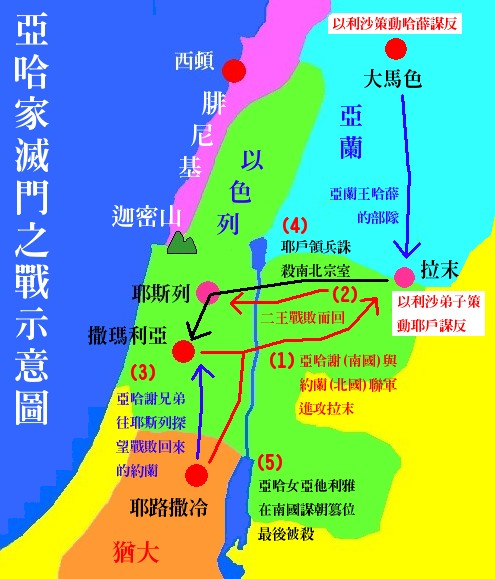
\includegraphics[width=5in]{BLiShiFigs/map_08}
\caption{耶戶}
\label{fig:sub1}
\end{figure}
在那些日子，耶和華才割裂以色列國，使哈薛攻擊以色列的境界， 33 乃是約旦河東，基列全地，從靠近亞嫩谷邊的亞羅珥起，就是基列和巴珊的迦得人、魯本人、瑪拿西人之地。 34 耶戶其餘的事，凡他所行的和他的勇力，都寫在《以色列諸王記》上。 35 耶戶與他列祖同睡，葬在撒馬利亞。他兒子約哈斯接續他做王。 36 耶戶在撒馬利亞做以色列王二十八年。

\newpage
\section{南國猶大王諸王 11-12 }
\subsection{亞他利雅 11 }
\subsubsection{亞他利雅滅王室篡國位 11:1-3}
亞哈謝的母親亞她利雅見她兒子死了，就起來剿滅王室。 2 但約蘭王的女兒、亞哈謝的妹子約示巴將亞哈謝的兒子約阿施從那被殺的王子中偷出來，把他和他的乳母都藏在臥房裡，躲避亞她利雅，免得被殺。 3 約阿施和他的乳母藏在耶和華的殿裡六年。亞她利雅篡了國位。

\subsubsection{耶何耶大與眾立約誓輔王子 11:4-12}
\begin{table}[H]
\hspace{-5mm}
\centering
\begin{tabular}{p{12.cm}|p{5.5cm}}\hline
\multicolumn{1}{c}{耶何耶大}&\multicolumn{1}{c}{護衛兵/眾人}\\\hline
第七年，耶何耶大打發人叫迦利人(親兵)和護衛兵的眾百夫長來，領他們進了耶和華的殿，與他們立約，使他們在耶和華殿裡起誓，又將王的兒子指給他們看，吩咐他們說：「你們當這樣行：凡安息日進班的，三分之一要看守王宮，三分之一要在蘇珥門，三分之一要在護衛兵院的後門。這樣把守王宮，攔阻閒人。你們安息日所有出班的三分之二，要在耶和華的殿裡護衛王。各人手拿兵器，四圍護衛王，凡擅入你們班次的必當治死。王出入的時候，你們當跟隨他。」&眾百夫長就照著祭司耶何耶大一切所吩咐的去行，各帶所管安息日進班出班的人來見祭司耶何耶大。\\\hline
祭司便將耶和華殿裡所藏大衛王的槍和盾牌交給百夫長。&護衛兵手中各拿兵器在壇和殿那裡，從殿右直到殿左站在王子的四圍。\\\hline
祭司領王子出來，給他戴上冠冕，將律法書交給他，膏他做王。&眾人就拍掌說：「願王萬歲！」\\\hline
\end{tabular}
\end{table}


\subsubsection{亞他利雅被殺 11:13-16}
\begin{table}[H]
\hspace{-5mm}
\centering
\begin{tabular}{p{9.75cm}|p{7.75cm}}\hline
\multicolumn{1}{c}{亞她利雅}&\multicolumn{1}{c}{祭司/眾人}\\\hline
亞她利雅聽見護衛兵和民的聲音，就到民那裡，進耶和華的殿。看見王照例站在柱旁，百夫長和吹號的人侍立在王左右，國中的眾民歡樂、吹號，亞她利雅就撕裂衣服，喊叫說：「反了！反了！」&祭司耶何耶大吩咐管轄軍兵的百夫長說：「將她趕出班外，凡跟隨她的必用刀殺死。」因為祭司說：「不可在耶和華殿裡殺她。」眾兵就閃開讓她去，\\\hline
她從馬路上王宮去，便在那裡被殺。&\\\hline
\end{tabular}
\end{table}





\subsection{猶大王約阿施 11:21-12:21 }
\subsubsection{耶何耶大使王和民與耶和華立約 11:17-21 }
\begin{table}[H]
\hspace{-5mm}
\centering
\begin{tabular}{p{3.cm}|p{5.5cm}|p{8.5cm}}\hline
\multicolumn{1}{c}{立約}&\multicolumn{1}{c}{打碎壇和巴力像}&\multicolumn{1}{c}{約阿施登基}\\\hline
耶何耶大使王和民與耶和華立約，做耶和華的民，又使王與民立約。&於是國民都到巴力廟，拆毀了廟，打碎壇和像，又在壇前將巴力的祭司瑪坦殺了。祭司耶何耶大派官看守耶和華的殿，&又率領百夫長和迦利人(親兵)與護衛兵，以及國中的眾民，請王從耶和華殿下來，由護衛兵的門進入王宮。他就坐了王位。國民都歡樂，合城都安靜。眾人已將亞她利雅在王宮那裡用刀殺了。約阿施登基的時候年方七歲。\\\hline
\end{tabular}
\end{table}

\subsubsection{約阿施登基做猶大王 12:1-3 }
耶戶第七年，約阿施登基，在耶路撒冷做王四十年。他母親名叫西比亞，是別是巴人。 2 約阿施在祭司耶何耶大教訓他的時候，就行耶和華眼中看為正的事。 3 只是丘壇還沒有廢去，百姓仍在那裡獻祭燒香。

\subsubsection{吩咐祭司修理聖殿 12:4-16 }
\begin{table}[H]
\hspace{-5mm}
\centering
\begin{tabular}{p{7.25cm}|p{10.5cm}}\hline
\multicolumn{1}{c}{祭司仍未修理殿}&\multicolumn{1}{c}{修理耶和華殿的破壞之處}\\\hline
約阿施對眾祭司說：「凡奉到耶和華殿分別為聖之物所值通用的銀子，或各人當納的身價，或樂意奉到耶和華殿的銀子，你們當從所認識的人收了來修理殿的一切破壞之處。」無奈到了約阿施王二十三年祭司仍未修理殿的破壞之處。所以約阿施王召了大祭司耶何耶大和眾祭司來對他們說：「你們怎麼不修理殿的破壞之處呢？從今以後，你們不要從所認識的人再收銀子，要將所收的交出來，修理殿的破壞之處。」眾祭司答應不再收百姓的銀子，也不修理殿的破壞之處。&祭司耶何耶大取了一個櫃子，在櫃蓋上鑽了一個窟窿放於壇旁，在進耶和華殿的右邊。守門的祭司將奉到耶和華殿的一切銀子投在櫃裡。他們見櫃裡的銀子多了，便叫王的書記和大祭司上來，將耶和華殿裡的銀子數算包起來。把所平的銀子交給督工的，就是耶和華殿裡辦事的人。他們把銀子轉交修理耶和華殿的木匠和工人，並瓦匠,石匠，又買木料和鑿成的石頭修理耶和華殿的破壞之處，以及修理殿的各樣使用。但那奉到耶和華殿的銀子沒有用以做耶和華殿裡的銀杯,蠟剪,碗,號和別樣的金銀器皿，乃將那銀子交給督工的人修理耶和華的殿。且將銀子交給辦事的人轉交做工的人，不與他們算帳，因為他們辦事誠實。唯有贖愆祭、贖罪祭的銀子沒有奉到耶和華的殿都歸祭司。\\\hline
\end{tabular}
\end{table}


\subsubsection{亞蘭王哈薛攻打約阿施 12:17-18 }
那時，亞蘭王哈薛上來攻打迦特，攻取了，就定意上來攻打耶路撒冷。 18 猶大王約阿施將他列祖猶大王約沙法、約蘭、亞哈謝所分別為聖的物和自己所分別為聖的物，並耶和華殿與王宮府庫裡所有的金子，都送給亞蘭王哈薛，哈薛就不上耶路撒冷來了。

\subsubsection{約阿施被殺 12:19-21 }
約阿施其餘的事，凡他所行的，都寫在《猶大列王記》上。 20 約阿施的臣僕起來背叛，在下悉拉的米羅宮那裡將他殺了， 21 殺他的那臣僕就是示米押的兒子約撒甲和朔默的兒子約薩拔。眾人將他葬在大衛城他列祖的墳地裡。他兒子亞瑪謝接續他做王。


\section{北國以色列 13 }
\subsection{以色列王約哈斯 13:1-9}
\subsubsection{約哈斯登基效法耶羅波安行惡 13:1-3 }
猶大王亞哈謝的兒子約阿施二十三年，耶戶的兒子約哈斯在撒馬利亞登基，做以色列王十七年。 2 約哈斯行耶和華眼中看為惡的事，效法尼八的兒子耶羅波安使以色列人陷在罪裡的那罪，總不離開。 3 於是耶和華的怒氣向以色列人發作，將他們屢次交在亞蘭王哈薛和他兒子便哈達的手裡。 

\subsubsection{約哈斯受亞蘭人欺壓 13:4-7 }
4 約哈斯懇求耶和華，耶和華就應允他，因為見以色列人所受亞蘭王的欺壓。 5 耶和華賜給以色列人一位拯救者，使他們脫離亞蘭人的手，於是以色列人仍舊安居在家裡。 6 然而他們不離開耶羅波安家使以色列人陷在罪裡的那罪，仍然去行，並且在撒馬利亞留下亞舍拉。 7 亞蘭王滅絕約哈斯的民，踐踏他們如禾場上的塵沙，只給約哈斯留下五十馬兵、十輛戰車、一萬步兵。 

\subsubsection{約哈斯之死 13:8-9 }
約哈斯其餘的事，凡他所行的和他的勇力，都寫在《以色列諸王記》上。 9 約哈斯與他列祖同睡，葬在撒馬利亞。他兒子約阿施接續他做王。

\subsection{以色列王約阿施 13:10-25}
\subsubsection{約阿施做以色列王 13:10-13 }
猶大王約阿施三十七年，約哈斯的兒子約阿施在撒馬利亞登基，做以色列王十六年。 11 他行耶和華眼中看為惡的事，不離開尼八的兒子耶羅波安使以色列人陷在罪裡的一切罪，仍然去行。 12 約阿施其餘的事，凡他所行的和他與猶大王亞瑪謝爭戰的勇力，都寫在《以色列諸王記》上。 13 約阿施與他列祖同睡，耶羅波安坐了他的位。約阿施與以色列諸王一同葬在撒馬利亞。

\subsubsection{以利沙病预言約阿施打敗亞蘭人三次 13:14-19}
\begin{table}[H]
\hspace{-5mm}
\centering
\begin{tabular}{p{9.95cm}|p{7.5cm}}\hline
\multicolumn{1}{c}{亞她利雅}&\multicolumn{1}{c}{祭司/眾人}\\\hline
以利沙得了必死的病。&以色列王約阿施下來看他，伏在他臉上哭泣，說：「我父啊！我父啊！以色列的戰車馬兵啊！」\\\hline
以利沙對他說：「你取弓箭來。」&王就取了弓箭來。\\\hline
又對以色列王說：「你用手拿弓。」&王就用手拿弓。\\\hline
以利沙按手在王的手上，說：「你開朝東的窗戶。」&他就開了。\\\hline
以利沙說：「射箭吧。」&他就射箭。\\\hline
以利沙說：「這是耶和華的得勝箭就是戰勝亞蘭人的箭。因為你必在亞弗攻打亞蘭人直到滅盡他們。」以利沙又說：「取幾枝箭來。」&他就取了來。\\\hline
以利沙說：「打地吧。」&他打了三次，便止住了。\\\hline
神人向他發怒，說：「應當擊打五六次，就能攻打亞蘭人直到滅盡。現在只能打敗亞蘭人三次。」&\\\hline
\end{tabular}
\end{table}


\subsubsection{以利沙骸骨使死人復活 13:20-21 }
以利沙死了，人將他葬埋。到了新年，有一群摩押人犯境。 21 有人正葬死人，忽然看見一群人，就把死人拋在以利沙的墳墓裡。一碰著以利沙的骸骨，死人就復活，站起來了。

\subsubsection{以色列與亞蘭的爭戰 13:22-25}
約哈斯年間，亞蘭王哈薛屢次欺壓以色列人。 23 耶和華卻因與亞伯拉罕、以撒、雅各所立的約，仍施恩給以色列人，憐恤他們，眷顧他們，不肯滅盡他們，尚未趕逐他們離開自己面前。 24 亞蘭王哈薛死了，他兒子便哈達接續他做王。 25 從前哈薛和約阿施的父親約哈斯爭戰，攻取了些城邑，現在約哈斯的兒子約阿施三次打敗哈薛的兒子便哈達，就收回了以色列的城邑。


\section{南國猶大王亞瑪謝 14:1-22 }
\subsubsection{亞瑪謝做王29年 14:1-2 }
以色列王約哈斯的兒子約阿施第二年，猶大王約阿施的兒子亞瑪謝登基。 2 他登基的時候年二十五歲，在耶路撒冷做王二十九年。他母親名叫約耶但，是耶路撒冷人。

\subsubsection{亞瑪謝懲治殺父之人,殺以東人 14:3-7}
亞瑪謝行耶和華眼中看為正的事，但不如他祖大衛，乃效法他父約阿施一切所行的。 4 只是丘壇還沒有廢去，百姓仍在那裡獻祭燒香。 5 國一堅定，就把殺他父王的臣僕殺了； 6 卻沒有治死殺王之人的兒子，是照摩西律法書上耶和華所吩咐的說：「不可因子殺父，也不可因父殺子，各人要為本身的罪而死。」
亞瑪謝在鹽谷殺了以東人一萬，又攻取了西拉，改名叫約帖，直到今日。

\subsubsection{向約阿施索戰,敗於伯士麥 14:8-14 }
\begin{table}[H]
\hspace{-5mm}
\centering
\begin{tabular}{p{4.5cm}|p{13.cm}}\hline
\multicolumn{1}{c|}{猶大王亞瑪謝}&\multicolumn{1}{c}{以色列王約阿施}\\\hline
那時，亞瑪謝差遣使者去見耶戶的孫子、約哈斯的兒子以色列王約阿施，說：「你來，我們二人相見於戰場。」&以色列王約阿施差遣使者去見猶大王亞瑪謝，說：「黎巴嫩的蒺藜差遣使者去見黎巴嫩的香柏樹，說：『將你的女兒給我兒子為妻。』後來黎巴嫩有一個野獸經過，把蒺藜踐踏了。你打敗了以東人，就心高氣傲。你以此為榮耀，在家裡安居就罷了，為何要惹禍，使自己和猶大國一同敗亡呢？」\\\hline
亞瑪謝卻不肯聽這話。&於是以色列王約阿施上來，在猶大的伯示麥與猶大王亞瑪謝相見於戰場。\\\hline
猶大人敗在以色列人面前，各自逃回家裡去了。&以色列王約阿施在伯示麥擒住亞哈謝的孫子、約阿施的兒子猶大王亞瑪謝，就來到耶路撒冷，拆毀耶路撒冷的城牆，從以法蓮門直到角門，共四百肘。又將耶和華殿裡與王宮府庫裡所有的金銀和器皿都拿了去，並帶人去為質，就回撒馬利亞去了。\\\hline
\end{tabular}
\end{table}


\subsubsection{以色列王約阿施之死 14:15-16 }
約阿施其餘所行的事和他的勇力，並與猶大王亞瑪謝爭戰的事，都寫在《以色列諸王記》上。 16 約阿施與他列祖同睡，葬在撒馬利亞以色列諸王的墳地裡。他兒子耶羅波安接續他做王。

\subsubsection{亞瑪謝被叛黨殺死在拉吉 14:17-22 }
以色列王約哈斯的兒子約阿施死後，猶大王約阿施的兒子亞瑪謝又活了十五年。 18 亞瑪謝其餘的事都寫在《猶大列王記》上。 19 耶路撒冷有人背叛亞瑪謝，他就逃到拉吉，叛黨卻打發人到拉吉將他殺了。 20 人就用馬將他的屍首馱到耶路撒冷，葬在大衛城他列祖的墳地裡。 21 猶大眾民立亞瑪謝的兒子亞撒利雅(又名烏西雅)接續他父做王，那時他年十六歲。 22 亞瑪謝與他列祖同睡之後，亞撒利雅收回以拉他仍歸猶大，又重新修理。

\section{北國以色列王耶羅波安二世 14:23-29)}
\subsubsection{耶羅波安二世登基做王41年 14:23 }
猶大王約阿施的兒子亞瑪謝十五年，以色列王約阿施的兒子耶羅波安在撒馬利亞登基，做王四十一年。

\subsubsection{神借耶羅波安二世的手所實行的拯救 14:24-29}
他行耶和華眼中看為惡的事，不離開尼八的兒子耶羅波安使以色列人陷在罪裡的一切罪。 25 他收回以色列邊界之地，從哈馬口直到亞拉巴海，正如耶和華以色列的神藉他僕人迦特希弗人亞米太的兒子先知約拿所說的。 26 因為耶和華看見以色列人甚是艱苦，無論困住的、自由的，都沒有了，也無人幫助以色列人。 27 耶和華並沒有說要將以色列的名從天下塗抹，乃藉約阿施的兒子耶羅波安拯救他們。

28 耶羅波安其餘的事，凡他所行的和他的勇力，他怎樣爭戰，怎樣收回大馬士革和先前屬猶大的哈馬歸以色列，都寫在《以色列諸王記》上。 29 耶羅波安與他列祖以色列諸王同睡。他兒子撒迦利雅接續他做王。


\section{南國猶大王亞撒利雅 15:1-7 }
\subsubsection{亞撒利雅做王52年行神眼中看為正的事 15:1-3 }
以色列王耶羅波安二十七年，猶大王亞瑪謝的兒子亞撒利雅登基。 2 他登基的時候年十六歲，在耶路撒冷做王五十二年。他母親名叫耶可利雅，是耶路撒冷人。 3 亞撒利雅行耶和華眼中看為正的事，效法他父親亞瑪謝一切所行的。

\subsubsection{亞撒利雅長大麻風 15:4-5 }
只是丘壇還沒有廢去，百姓仍在那裡獻祭燒香。 5 耶和華降災於王，使他長大痲瘋直到死日，他就住在別的宮裡。他的兒子約坦管理家事，治理國民。

\subsubsection{亞撒利雅的兒子約坦登基 15:6-7 }
亞撒利雅其餘的事，凡他所行的，都寫在《猶大列王記》上。 7 亞撒利雅與他列祖同睡，葬在大衛城他列祖的墳地裡。他兒子約坦接續他做王。

\section{北國以色列諸王 15:8-31 }
\subsection{耶羅波安的兒子撒迦利亞做王六個月 15:8-12 }
猶大王亞撒利雅三十八年，耶羅波安的兒子撒迦利雅在撒馬利亞做以色列王六個月。 9 他行耶和華眼中看為惡的事，效法他列祖所行的，不離開尼八的兒子耶羅波安使以色列人陷在罪裡的那罪。 10 雅比的兒子沙龍背叛他，在百姓面前擊殺他，篡了他的位。 11 撒迦利雅其餘的事都寫在《以色列諸王記》上。 12 這是從前耶和華應許耶戶說：「你的子孫必坐以色列的國位，直到四代。」這話果然應驗了。

\subsection{雅比的兒子沙龍做王一個月 15:13-16 }
猶大王烏西雅(亞撒利雅)三十九年，雅比的兒子沙龍登基，在撒馬利亞做王一個月。 14 迦底的兒子米拿現從得撒上撒馬利亞，殺了雅比的兒子沙龍，篡了他的位。 15 沙龍其餘的事和他背叛的情形都寫在《以色列諸王記》上。 16 那時米拿現從得撒起攻打提斐薩和其四境，擊殺城中一切的人，剖開其中所有的孕婦，都因他們沒有給他開城。

\subsection{迦底的兒子米拿現做王10年 15:17-22 }
猶大王亞撒利雅三十九年，迦底的兒子米拿現登基，在撒馬利亞做以色列王十年。 18 他行耶和華眼中看為惡的事，終身不離開尼八的兒子耶羅波安使以色列人陷在罪裡的那罪。 19 亞述王普勒來攻擊以色列國，米拿現給他一千他連得銀子，請普勒幫助他堅定國位。 20 米拿現向以色列一切大富戶索要銀子，使他們各出五十舍客勒，就給了亞述王。於是亞述王回去，不在國中停留。 21 米拿現其餘的事，凡他所行的，都寫在《以色列諸王記》上。 22 米拿現與他列祖同睡。他兒子比加轄接續他做王。

\subsection{米拿現的兒子比加轄做王2年 15:23-26 }
猶大王亞撒利雅五十年，米拿現的兒子比加轄在撒馬利亞登基，做以色列王二年。 24 他行耶和華眼中看為惡的事，不離開尼八的兒子耶羅波安使以色列人陷在罪裡的那罪。 25 比加轄的將軍，利瑪利的兒子比加背叛他，在撒馬利亞王宮裡的衛所殺了他，亞珥歌伯和亞利耶並基列的五十人幫助比加。比加擊殺他，篡了他的位。 26 比加轄其餘的事，凡他所行的，都寫在《以色列諸王記》上。

\subsection{利瑪利的兒子比加做王20年 15:27-31 }
猶大王亞撒利雅五十二年，利瑪利的兒子比加在撒馬利亞登基，做以色列王二十年。 28 他行耶和華眼中看為惡的事，不離開尼八的兒子耶羅波安使以色列人陷在罪裡的那罪。

29 以色列王比加年間，亞述王提革拉毗列色來奪了以雲、亞伯伯瑪迦、亞挪、基低斯、夏瑣、基列、加利利和拿弗他利全地，將這些地方的居民都擄到亞述去了。 30 烏西雅的兒子約坦二十年，以拉的兒子何細亞背叛利瑪利的兒子比加，擊殺他，篡了他的位。 31 比加其餘的事，凡他所行的，都寫在《以色列諸王記》上。

\section{南國猶大王諸王 15:32-16:20 }
\subsection{烏西雅的兒子約坦做王16年 15:32-38 }
以色列王利瑪利的兒子比加第二年，猶大王烏西雅的兒子約坦登基。 33 他登基的時候年二十五歲，在耶路撒冷做王十六年。他母親名叫耶路沙，是撒督的女兒。 34 約坦行耶和華眼中看為正的事，效法他父親烏西雅一切所行的。 35 只是丘壇還沒有廢去，百姓仍在那裡獻祭燒香。約坦建立耶和華殿的上門。 36 約坦其餘的事，凡他所行的，都寫在《猶大列王記》上。 37 在那些日子，耶和華才使亞蘭王利汛和利瑪利的兒子比加去攻擊猶大。 38 約坦與他列祖同睡，葬在他祖大衛城他列祖的墳地裡。他兒子亞哈斯接續他做王。

\subsection{約坦的兒子亞哈斯王 16:1-20 }
\subsubsection{亞哈斯做猶大王16年 16:1-4}
\begin{table}[H]
\hspace{-5mm}
\centering
\begin{tabular}{p{7.75cm}|p{9.5cm}}\hline
\multicolumn{1}{c|}{做猶大王16年}&\multicolumn{1}{c}{效法以色列諸王和外邦人}\\\hline
\multirow{2}{8.1cm}{利瑪利的兒子比加十七年，猶大王約坦的兒子亞哈斯登基。他登基的時候年二十歲，在耶路撒冷做王十六年。}&不像他祖大衛行耶和華他神眼中看為正的事，卻效法\textcolor{blue}{以色列諸王}所行的，\\\cline{2-2}
&又照著耶和華從以色列人面前趕出的\textcolor{blue}{外邦人}所行可憎的事，使他的兒子經火，並在丘壇上、山岡上、各青翠樹下獻祭燒香。\\\hline
\end{tabular}
\end{table}


\subsubsection{亞蘭王以色列王合攻耶路撒冷 16:5-6}
亞蘭王利汛和以色列王利瑪利的兒子比加上來攻打耶路撒冷，圍困亞哈斯，卻不能勝他。 6 當時亞蘭王利汛收回以拉他歸於亞蘭，將猶大人從以拉他趕出去。亞蘭人(以東人)就來到以拉他，住在那裡，直到今日。

\subsubsection{求救於亞述王,把亞蘭居民擄到吉珥 16:7-9}
亞哈斯差遣使者去見亞述王提革拉毗列色，說：「我是你的僕人，你的兒子。現在亞蘭王和以色列王攻擊我，求你來救我脫離他們的手。」 8 亞哈斯將耶和華殿裡和王宮府庫裡所有的金銀都送給亞述王為禮物。 9 亞述王應允了他，就上去攻打大馬士革，將城攻取，殺了利汛，把居民擄到吉珥。


\subsubsection{擅更祭壇祭禮 16:10-16}
\begin{table}[H]
\hspace{-5mm}
\centering
\begin{tabular}{p{6.1cm}|p{11.25cm}}\hline
\multicolumn{1}{c|}{建築大馬士革壇}&\multicolumn{1}{c}{在大馬士革獻祭,用銅壇用求問耶和華}\\\hline
\multirow{2}{6.2cm}{那亞哈斯王上大馬士革去迎接亞述王提革拉毗列色，在大馬士革看見一座壇，就照壇的規模,樣式,做法畫了圖樣送到祭司烏利亞那裡。祭司烏利亞照著亞哈斯王從大馬士革送來的圖樣，在亞哈斯王沒有從大馬士革回來之先建築一座壇。}
&王從大馬士革回來看見壇，就近前來，在壇上獻祭，燒燔祭、素祭，澆奠祭，將平安祭牲的血灑在壇上。又將耶和華面前的銅壇，從耶和華殿和新壇的中間搬到新壇的北邊。亞哈斯王吩咐祭司烏利亞說："早晨的燔祭，晚上的素祭，王的燔祭、素祭，國內眾民的燔祭、素祭、奠祭都要燒在大壇上，燔祭牲和平安祭牲的血也要灑在這壇上，\\\cline{2-2}
&只是銅壇我要用以求問耶和華"祭司烏利亞就照著亞哈斯王所吩咐的行了\\\hline
\end{tabular}
\end{table}



\subsubsection{私改挪移銅盆銅海，挪移聖殿廊子 16:17-20}
亞哈斯王打掉盆座四面鑲著的心子，把盆從座上挪下來，又將銅海從馱海的銅牛上搬下來，放在鋪石地。 18 又因亞述王的緣故，將耶和華殿為安息日所蓋的廊子和王從外入殿的廊子挪移，圍繞耶和華的殿。 19 亞哈斯其餘所行的事都寫在《猶大列王記》上。 20 亞哈斯與他列祖同睡，葬在大衛城他列祖的墳地裡。他兒子希西家接續他做王。


\section{北國以色列亡國 17 }
\subsection{以拉的兒子何細亞 17:1-6}
\subsubsection{何細亞王做以色列王九年 17:1-6}
猶大王亞哈斯十二年，以拉的兒子何細亞在撒馬利亞登基，做以色列王九年。 2 他行耶和華眼中看為惡的事，只是不像在他以前的以色列諸王。 3 亞述王撒縵以色上來攻擊何細亞，何細亞就服侍他，給他進貢。 4 何細亞背叛，差人去見埃及王梭，不照往年所行的與亞述王進貢。亞述王知道了，就把他鎖禁，囚在監裡。亞述王上來攻擊以色列遍地，上到撒馬利亞，圍困三年。 6 何細亞第九年，亞述王攻取了撒馬利亞，將以色列人擄到亞述，把他們安置在哈臘與歌散的哈博河邊，並瑪代人的城邑。


\subsubsection{以色列人所犯的罪 17:7-23}
\subsubsubsection{敬畏隨從外邦人神 17:7-12}
這是因以色列人得罪那領他們出埃及地，脫離埃及王法老手的耶和華他們的神，去敬畏別神， 8 隨從耶和華在他們面前所趕出外邦人的風俗和以色列諸王所立的條規。 9 以色列人暗中行不正的事，違背耶和華他們的神，在他們所有的城邑，從瞭望樓直到堅固城，建築丘壇； 10 在各高岡上、各青翠樹下立柱像和木偶； 11 在丘壇上燒香，效法耶和華在他們面前趕出的外邦人所行的；又行惡事，惹動耶和華的怒氣； 12 且侍奉偶像，就是耶和華警戒他們不可行的。

\subsubsubsection{不聽從眾先知的勸誡 17:13-18} 
13 但耶和華藉眾先知、先見勸誡以色列人和猶大人說：「當離開你們的惡行，謹守我的誡命、律例，遵行我吩咐你們列祖並藉我僕人眾先知所傳給你們的律法。」 14 他們卻不聽從，竟硬著頸項，效法他們列祖，不信服耶和華他們的神， 15 厭棄他的律例和他與他們列祖所立的約並勸誡他們的話，隨從虛無的神，自己成為虛妄，效法周圍的外邦人，就是耶和華囑咐他們不可效法的。 16 離棄耶和華他們神的一切誡命，為自己鑄了兩個牛犢的像，立了亞舍拉，敬拜天上的萬象，侍奉巴力； 17 又使他們的兒女經火，用占卜，行法術，賣了自己行耶和華眼中看為惡的事，惹動他的怒氣。 18 所以耶和華向以色列人大大發怒，從自己面前趕出他們，只剩下猶大一個支派。

\subsubsubsection{神厭棄使以色列全族受苦 17:19-23}
猶大人也不遵守耶和華他們神的誡命，隨從以色列人所立的條規。 20 耶和華就厭棄以色列全族，使他們受苦，把他們交在搶奪他們的人手中，以致趕出他們離開自己面前， 21 將以色列國從大衛家奪回，他們就立尼八的兒子耶羅波安做王。耶羅波安引誘以色列人不隨從耶和華，陷在大罪裡。 22 以色列人犯耶羅波安所犯的一切罪，總不離開， 23 以致耶和華從自己面前趕出他們，正如藉他僕人眾先知所說的。這樣，以色列人從本地被擄到亞述，直到今日。


\subsubsection{獅子咬死一些遷居撒瑪利亞的諸族 17:24-28 }
\begin{table}[H]
\hspace{-10mm}
\centering
\begin{tabular}{p{10.75cm}|p{6.cm}}\hline\hline
\multicolumn{1}{c|}{獅子咬死不敬畏耶和華的諸族}&\multicolumn{1}{c}{擄去的撒馬利亞祭司回伯特利}\\\hline
亞述王從巴比倫,古他,亞瓦,哈馬和西法瓦音遷移人來，安置在撒馬利亞的城邑代替以色列人。他們就得了撒馬利亞住在其中。他們才住那裡的時候不敬畏耶和華，所以耶和華叫獅子進入他們中間咬死了些人。有人告訴亞述王說：「你所遷移安置在撒馬利亞各城的那些民不知道那地之神的規矩，所以那神叫獅子進入他們中間咬死他們。」&亞述王就吩咐說：「叫所擄來的祭司回去一個，使他住在那裡，將那地之神的規矩指教那些民。」於是有一個從撒馬利亞擄去的祭司回來，住在伯特利，指教他們怎樣敬畏耶和華。\\\hline
\end{tabular}
\end{table}


\subsubsection{居民雜居，信仰混亂 17:29-41 }
\begin{table}[H]
\centering
\begin{tabular}{p{3.5cm}||p{13.5cm}}\hline\hline
\multicolumn{1}{c|}{信仰混亂}&\multicolumn{1}{c}{懼怕耶和華，又侍奉自己的神}\\\hline
\multirow{3}{3.6cm}{然而各族之人在所住的城裡各為自己製造神像，安置在撒馬利亞人所造有丘壇的殿中。巴比倫人造疏割比訥像，古他人造匿甲像，哈馬人造亞示瑪像，亞瓦人造匿哈和他珥他像，西法瓦音人用火焚燒兒女獻給西法瓦音的神亞得米勒和亞拿米勒。}
&他們懼怕耶和華，也從他們中間立丘壇的祭司，為他們在有丘壇的殿中獻祭。他們又懼怕耶和華，又侍奉自己的神，從何邦遷移，就隨何邦的風俗。他們直到如今仍照先前的風俗去行，不專心敬畏耶和華，不全守自己的規矩、典章，也不遵守耶和華吩咐雅各後裔的律法、誡命；雅各，就是從前耶和華起名叫以色列的。\\\cline{2-2}
&耶和華曾與他們立約，囑咐他們說：「不可敬畏別神，不可跪拜侍奉他，也不可向他獻祭。但那用大能和伸出來的膀臂領你們出埃及地的耶和華，你們當敬畏、跪拜，向他獻祭。他給你們寫的律例、典章、律法、誡命，你們應當永遠謹守遵行，不可敬畏別神。我耶和華與你們所立的約，你們不可忘記，也不可敬畏別神，但要敬畏耶和華你們的神，他必救你們脫離一切仇敵的手。」\\\cline{2-2} 
&他們卻不聽從，仍照先前的風俗去行。如此，這些民又懼怕耶和華，又侍奉他們的偶像。他們子子孫孫也都照樣行，效法他們的祖宗，直到今日。\\\hline
\end{tabular}
\end{table}


\section{南國猶大王諸王 18-25 }

\subsection{亞哈斯的兒子希西家 18-20 }
\subsubsection{希西家做王29年 18:1-2}
以色列王以拉的兒子何細亞第三年，猶大王亞哈斯的兒子希西家登基。 2 他登基的時候年二十五歲，在耶路撒冷做王二十九年。他母親名叫亞比，是撒迦利雅的女兒。

\subsubsection{專心遵守耶和華的命令 18:3-8}
\begin{table}[H]
\centering
\begin{tabular}{p{6.5cm}|p{6.cm}|p{4.cm}}\hline\hline
\multicolumn{1}{c|}{行耶和華看為正的事}&\multicolumn{1}{c}{倚靠耶和華}&\multicolumn{1}{c}{背叛亞述，攻擊非利士}\\\hline
希西家行耶和華眼中看為正的事，效法他祖大衛一切所行的。他廢去丘壇，毀壞柱像，砍下木偶，打碎摩西所造的銅蛇，因為到那時以色列人仍向銅蛇燒香；希西家叫銅蛇為銅塊(人稱銅蛇為銅像)。
&希西家倚靠耶和華以色列的神，在他前後的猶大列王中沒有一個及他的。因為他專靠耶和華，總不離開，謹守耶和華所吩咐摩西的誡命。耶和華與他同在，他無論往何處去盡都亨通。
&他背叛，不肯侍奉亞述王。希西家攻擊非利士人，直到加沙並加沙的四境，從瞭望樓到堅固城。\\\hline
\end{tabular}
\end{table}




\subsubsection{希西家王第四年以色列亡於亞述 18:9-12}
希西家王第四年，就是以色列王以拉的兒子何細亞第七年，亞述王撒縵以色上來圍困撒馬利亞。 10 過了三年，就攻取了城。希西家第六年，以色列王何細亞第九年，撒馬利亞被攻取了。 11 亞述王將以色列人擄到亞述，把他們安置在哈臘與歌散的哈博河邊並瑪代人的城邑； 12 都因他們不聽從耶和華他們神的話，違背他的約，就是耶和華僕人摩西吩咐他們所當守的。

\subsubsection{希西家王十四年,神救助南國脫離亞述王的手 18:13-19:37}

\begin{table}[!hbp]
\centering
\begin{tabular}{|p{2cm}||p{13cm}|}
\hline
\hline
  地點   & 事件  \\\hline\hline
 猶大堅固城  & 希西家王十四年，亞述王西拿基立攻擊猶大的一切堅固城，將城攻取  \\\hline
拉吉 & 希西家差人往拉吉去見亞述王賠款求和   \\\hline
耶路撒冷    & 亞述王從拉吉差遣大軍攻打耶路撒冷 \\\hline
上池水溝旁    & 拉伯沙基向家宰以利亞敬，並書記舍伯那和史官約亞挑釁 \\\hline
希西家那裡    & 家宰以利亞敬，並書記舍伯那和史官約亞向希西家回复 \\\hline
耶和華的殿    & 希西家王聽見，就撕裂衣服，披上麻布，進了耶和華的殿 \\\hline
先知以賽亞    &希西家差遣以利亞敬,舍伯那,祭司中的長老，都披上麻布，去見亞摩斯的兒子先知以賽亞,以賽亞预言亞述王失败 \\\hline
立拿    & 拉伯沙基回去，正遇見亞述王攻打立拿，原來他早聽見亞述王拔營離開拉吉 \\\hline
  耶路撒冷   & 亞述王托使者给希西家带信 \\\hline
耶和華的殿    & 希西家從使者手裡接過書信來，看完了，就上耶和華的殿，將書信在耶和華面前展開祷告 \\\hline
以賽亞    & 亞摩斯的兒子以賽亞就打發人去見希西家预言亚述必败 \\\hline
亞述營    & 當夜，耶和華的使者出去，在亞述營中殺了十八萬五千人 \\\hline
尼尼微    & 亞述王西拿基立就拔營回去，住在尼尼微。 \\\hline
尼斯洛廟    & 亞述王在尼斯洛廟裡叩拜,他兒子亞得米勒和沙利色用刀殺了他 \\\hline
\end{tabular}
\caption{希西家脫離亞述王的手}
\end{table}

\subsubsubsection{西拿基立攻取猶大諸邑,罰猶大王金銀 18:13-16}
\begin{table}[H]
\centering
\begin{tabular}{p{5.75cm}|p{11.75cm}}\hline\hline
\multicolumn{1}{c|}{亞述王西拿基立}&\multicolumn{1}{c}{猶大王希西家}\\\hline
希西家王十四年，亞述王西拿基立上來攻擊猶大的一切堅固城，將城攻取。
&猶大王希西家差人往拉吉去見亞述王，說：「我有罪了，求你離開我。凡你罰我的，我必承當。」\\\hline
於是亞述王罰猶大王希西家銀子三百他連得，金子三十他連得。&希西家就把耶和華殿裡和王宮府庫裡所有的銀子都給了他。那時猶大王希西家將耶和華殿門上的金子和他自己包在柱上的金子都刮下來，給了亞述王。\\\hline
\end{tabular}
\end{table}


\subsubsubsection{拉伯沙基用猶大語狂言耶和華 18:17-37}
\begin{table}[H]
\centering
\begin{tabular}{p{1.9cm}|p{2.75cm}|p{12.cm}}\hline\hline
\multicolumn{1}{c|}{亞述代表}&\multicolumn{1}{c|}{以利亞敬等}&\multicolumn{1}{c|}{拉伯沙基狂言}\\\hline
\multirow{4}{2.1cm}{亞述王從拉吉差遣他珥探、拉伯撒利和拉伯沙基率領大軍往耶路撒冷，到希西家王那裡去。他們上到耶路撒冷，就站在上池的水溝旁，在漂布地的大路上。他們呼叫王的時候，}
&\multirow{4}{2.9cm}{就有希勒家的兒子家宰以利亞敬，並書記舍伯那和亞薩的兒子史官約亞，出來見他們。希勒家的兒子以利亞敬和舍伯那並約亞對拉伯沙基說：「求你用亞蘭言語和僕人說話，因為我們懂得。不要用猶大言語和我們說話，達到城上百姓的耳中。」}&拉伯沙基說：「我主差遣我來，豈是單對你和你的主說這些話嗎？不也是對這些坐在城上，要與你們一同吃自己糞喝自己尿的人說嗎？」\\\cline{3-3}
&&於是拉伯沙基站著，用猶大言語大聲喊著說：「你們當聽亞述大王的話！王如此說：『你們不要被希西家欺哄了，因他不能救你們脫離我的手。也不要聽希西家使你們倚靠耶和華說：「耶和華必要拯救我們，這城必不交在亞述王的手中。」』不要聽希西家的話，\\\cline{3-3}
&&因亞述王如此說：『你們要與我和好，出來投降我，各人就可以吃自己葡萄樹和無花果樹的果子，喝自己井裡的水。等我來領你們到一個地方，與你們本地一樣，就是有五穀和新酒之地，有糧食和葡萄園之地，有橄欖樹和蜂蜜之地，好使你們存活，不至於死。\\\cline{3-3}
&&希西家勸導你們說：「耶和華必拯救我們。」你們不要聽他的話。列國的神，有哪一個救他本國脫離亞述王的手呢？哈馬、亞珥拔的神在哪裡呢？西法瓦音、希拿、以瓦的神在哪裡呢？他們曾救撒馬利亞脫離我的手嗎？這些國的神有誰曾救自己的國脫離我的手呢？難道耶和華能救耶路撒冷脫離我的手嗎？』」\\\hline
\end{tabular}
\end{table}



\subsubsubsection{希西家聞之而憂，差人见以賽亞得慰詞 18:36-19:7}
\begin{table}[H]
\hspace{-8mm}
\centering
\begin{tabular}{p{3.9cm}|p{8.75cm}|p{4.5cm}}\hline\hline
\multicolumn{1}{c|}{希西家聞拉伯沙基狂言}&\multicolumn{1}{c|}{希西家進神殿，差人求先知}&\multicolumn{1}{c}{以賽亞慰詞}\\\hline
\multirow{4}{4.1cm}{百姓靜默不言，並不回答一句，因為王曾吩咐說：「不要回答他。」當下，希勒家的兒子家宰以利亞敬，和書記舍伯那並亞薩的兒子史官約亞，都撕裂衣服來到希西家那裡，將拉伯沙基的話告訴了他。}
&希西家王聽見，就撕裂衣服，披上麻布，進了耶和華的殿。 &\multirow{4}{4.67cm}{希西家王的臣僕就去見以賽亞。以賽亞對他們說：「要這樣對你們的主人說：『耶和華如此說：你聽見亞述王的僕人褻瀆我的話，不要懼怕。我必驚動 （使靈進入）他的心，他要聽見風聲，就歸回本地，我必使他在那裡倒在刀下。』」」}\\\cline{2-2}

&使家宰以利亞敬和書記舍伯那並祭司中的長老都披上麻布，去見亞摩斯的兒子先知以賽亞，對他說：「希西家如此說：今日是急難、責罰、凌辱的日子，就如婦人將要生產嬰孩，卻沒有力量生產。或者耶和華你的神聽見拉伯沙基的一切話，就是他主人亞述王打發他來辱罵永生神的話，耶和華你的神聽見這話就發斥責。故此，求你為餘剩的民揚聲禱告。」&\\\hline
\end{tabular}
\end{table}



\subsubsubsection{亞述王又打發使者达信恐吓希西家 19:8-13}
拉伯沙基回去，正遇見亞述王攻打立拿，原來他早聽見亞述王拔營離開拉吉。 9 亞述王聽見人論古實王特哈加說：「他出來要與你爭戰。」於是亞述王又打發使者去見希西家，吩咐他們說： 10 「你們對猶大王希西家如此說：不要聽你所倚靠的神欺哄你說：『耶路撒冷必不交在亞述王的手中。』 11 你總聽說亞述諸王向列國所行的，乃是盡行滅絕，難道你還能得救嗎？ 12 我列祖所毀滅的，就是歌散、哈蘭、利色和屬提拉撒的伊甸人，這些國的神何曾拯救這些國呢？ 13 哈馬的王、亞珥拔的王、西法瓦音城的王、希拿和以瓦的王都在哪裡呢？」

\subsubsubsection{希西家上耶和華的殿祈禱 19:14-19}
希西家從使者手裡接過書信來，看完了，就上耶和華的殿，將書信在耶和華面前展開。 15 希西家向耶和華禱告說：「坐在二基路伯上耶和華以色列的神啊，你是天下萬國的神，你曾創造天地。 16 耶和華啊，求你側耳而聽！耶和華啊，求你睜眼而看！要聽西拿基立打發使者來辱罵永生神的話。 17 耶和華啊，亞述諸王果然使列國和列國之地變為荒涼， 18 將列國的神像都扔在火裡，因為它本不是神，乃是人手所造的，是木頭、石頭的，所以滅絕它。 19 耶和華我們的神啊，現在求你救我們脫離亞述王的手，使天下萬國都知道，唯獨你耶和華是神。」

\subsubsubsection{以賽亞預言耶和華拯救 19:20-34}
亞摩斯的兒子以賽亞就打發人去見希西家，說：「耶和華以色列的神如此說：你既然求我攻擊亞述王西拿基立，我已聽見了。 21 耶和華論他這樣說：『錫安的處女藐視你，嗤笑你，耶路撒冷的女子向你搖頭。 22 你辱罵誰，褻瀆誰？揚起聲來，高舉眼目攻擊誰呢？乃是攻擊以色列的聖者！ 23 你藉你的使者辱罵主，並說：「我率領許多戰車上山頂，到黎巴嫩極深之處，我要砍伐其中高大的香柏樹和佳美的松樹，我必上極高之處，進入肥田的樹林。 24 我已經在外邦挖井喝水，我必用腳掌踏乾埃及的一切河。」』

25 「耶和華說：『我早先所做的，古時所立的，就是現在藉你使堅固城荒廢，變為亂堆，這事你豈沒有聽見嗎？ 26 所以其中的居民力量甚小，驚惶羞愧，他們像野草，像青菜，如房頂上的草，又如未長成而枯乾的禾稼。 27 你坐下，你出去，你進來，你向我發烈怒，我都知道。 28 因你向我發烈怒，又因你狂傲的話達到我耳中，我就要用鉤子鉤上你的鼻子，把嚼環放在你口裡，使你從你來的路轉回去。』
以色列人哪，我賜你們一個證據：你們今年要吃自生的，明年也要吃自長的，至於後年，你們要耕種收割，栽植葡萄園，吃其中的果子。 30 猶大家所逃脫餘剩的，仍要往下扎根，向上結果。 31 必有餘剩的民從耶路撒冷而出，必有逃脫的人從錫安山而來。耶和華的熱心必成就這事。 32 所以耶和華論亞述王如此說：他必不得來到這城，也不在這裡射箭，不得拿盾牌到城前，也不築壘攻城。 33 他從哪條路來，必從哪條路回去，必不得來到這城。這是耶和華說的。 34 因我為自己的緣故，又為我僕人大衛的緣故，必保護拯救這城。」

\subsubsubsection{耶和華的使者殺了十八萬五千亞述人 19:35-37}
當夜，耶和華的使者出去，在亞述營中殺了十八萬五千人。清早有人起來，一看，都是死屍了。 36 亞述王西拿基立就拔營回去，住在尼尼微。 37 一日，在他的神尼斯洛廟裡叩拜，他兒子亞得米勒和沙利色用刀殺了他，就逃到亞拉臘地。他兒子以撒哈頓接續他做王。

\subsubsection{希西家重病得醫治 20:1-11}
那時，希西家病得要死。亞摩斯的兒子先知以賽亞去見他，對他說：「耶和華如此說：你當留遺命於你的家，因為你必死，不能活了。」 2 希西家就轉臉朝牆，禱告耶和華說： 3 「耶和華啊，求你記念我在你面前怎樣存完全的心，按誠實行事，又做你眼中所看為善的。」希西家就痛哭了。 4 以賽亞出來，還沒有到中院(城)，耶和華的話就臨到他說： 5 「你回去告訴我民的君希西家說：『耶和華你祖大衛的神如此說：我聽見了你的禱告，看見了你的眼淚。我必醫治你，到第三日，你必上到耶和華的殿。 6 我必加增你十五年的壽數，並且我要救你和這城脫離亞述王的手。我為自己和我僕人大衛的緣故，必保護這城。』」 7 以賽亞說：「當取一塊無花果餅來。」人就取了來，貼在瘡上，王便痊癒了。

8 希西家問以賽亞說：「耶和華必醫治我，到第三日我能上耶和華的殿，有什麼兆頭呢？」 9 以賽亞說：「耶和華必成就他所說的。這是他給你的兆頭：你要日影向前進十度呢？是要往後退十度呢？」 10 希西家回答說：「日影向前進十度容易，我要日影往後退十度。」 11 先知以賽亞求告耶和華，耶和華就使亞哈斯的日晷向前進的日影往後退了十度。

\subsubsection{希西家向巴比倫的使者炫耀財富 20:12-19}
那時，巴比倫王巴拉但的兒子比羅達巴拉但聽見希西家病而痊癒，就送書信和禮物給他。 13 希西家聽從使者的話，就把他寶庫的金子、銀子、香料、貴重的膏油和他武庫的一切軍器，並他所有的財寶，都給他們看。他家中和他全國之內，希西家沒有一樣不給他們看的。 14 於是先知以賽亞來見希西家王，問他說：「這些人說什麼？他們從哪裡來見你？」希西家說：「他們從遠方的巴比倫來。」 15 以賽亞說：「他們在你家裡看見了什麼？」希西家說：「凡我家中所有的，他們都看見了，我財寶中沒有一樣不給他們看的。」

16 以賽亞對希西家說：「你要聽耶和華的話： 17 日子必到，凡你家裡所有的，並你列祖積蓄到如今的，都要被擄到巴比倫去，不留下一樣。這是耶和華說的。 18 並且從你本身所生的眾子，其中必有被擄去，在巴比倫王宮裡當太監的。」 19 希西家對以賽亞說：「你所說耶和華的話甚好。若在我的年日中有太平和穩固的景況，豈不是好嗎？」

\subsubsection{希西家之死 20:20-21}
希西家其餘的事和他的勇力，他怎樣挖池挖溝，引水入城，都寫在《猶大列王記》上。 21 希西家與他列祖同睡。他兒子瑪拿西接續他做王。

\subsection{瑪拿西 21:1-18 }
\subsubsection{瑪拿西登基做王55年 21:1}
瑪拿西登基的時候年十二歲，在耶路撒冷做王五十五年。他母親名叫協西巴。

\subsubsection{瑪拿西行耶和华眼中看为恶的事 21:2-9}
 2 瑪拿西行耶和華眼中看為惡的事，效法耶和華在以色列人面前趕出的外邦人所行可憎的事， 3 重新建築他父希西家所毀壞的丘壇，又為巴力築壇，做亞舍拉像，效法以色列王亞哈所行的，且敬拜侍奉天上的萬象， 4 在耶和華殿宇中築壇，耶和華曾指著這殿說：「我必立我的名在耶路撒冷。」 5 他在耶和華殿的兩院中為天上的萬象築壇， 6 並使他的兒子經火，又觀兆，用法術，立交鬼的和行巫術的，多行耶和華眼中看為惡的事，惹動他的怒氣， 7 又在殿內立雕刻的亞舍拉像。耶和華曾對大衛和他兒子所羅門說：「我在以色列眾支派中所選擇的耶路撒冷和這殿，必立我的名直到永遠。 8 以色列人若謹守遵行我一切所吩咐他們的和我僕人摩西所吩咐他們的一切律法，我就不再使他們挪移，離開我所賜給他們列祖之地。」 9 他們卻不聽從。瑪拿西引誘他們行惡，比耶和華在以色列人面前所滅的列國更甚。

\subsubsection{耶和華藉他僕人眾先知预言棄掉所餘剩的子民 21:10-16}
耶和華藉他僕人眾先知說： 11 「因猶大王瑪拿西行這些可憎的惡事比先前亞摩利人所行的更甚，使猶大人拜他的偶像陷在罪裡， 12 所以耶和華以色列的神如此說：我必降禍於耶路撒冷和猶大，叫一切聽見的人無不耳鳴。 13 我必用量撒馬利亞的準繩和亞哈家的線砣，拉在耶路撒冷上；必擦淨耶路撒冷，如人擦盤將盤倒扣。 14 我必棄掉所餘剩的子民(產業)，把他們交在仇敵手中，使他們成為一切仇敵擄掠之物。 15 是因他們自從列祖出埃及直到如今，常行我眼中看為惡的事，惹動我的怒氣。」

16 瑪拿西行耶和華眼中看為惡的事，使猶大人陷在罪裡，又流許多無辜人的血，充滿了耶路撒冷，從這邊直到那邊。

\subsubsection{瑪拿西與他列祖同睡 21:17-18}
瑪拿西其餘的事，凡他所行的和他所犯的罪，都寫在《猶大列王記》上。 18 瑪拿西與他列祖同睡，葬在自己宮院烏撒的園內。他兒子亞們接續他做王。

\subsection{亞們 21:19-26 }
亞們登基的時候年二十二歲，在耶路撒冷做王二年。他母親名叫米舒利密，是約提巴人哈魯斯的女兒。 20 亞們行耶和華眼中看為惡的事，與他父親瑪拿西所行的一樣， 21 行他父親一切所行的，敬奉他父親所敬奉的偶像， 22 離棄耶和華他列祖的神，不遵行耶和華的道。 23 亞們王的臣僕背叛他，在宮裡殺了他。 24 但國民殺了那些背叛亞們王的人，立他兒子約西亞接續他做王。 25 亞們其餘所行的事都寫在《猶大列王記》上。 26 亞們葬在烏撒的園內自己的墳墓裡。他兒子約西亞接續他做王。

\subsection{約西亞 22:1-23:30 }
\subsubsection{約西亞登基做王31年 22:1-2}
約西亞登基的時候年八歲，在耶路撒冷做王三十一年。他母親名叫耶底大，是波斯加人亞大雅的女兒。 2 約西亞行耶和華眼中看為正的事，行他祖大衛一切所行的，不偏左右。

\subsubsection{約西亞吩咐修理圣殿 22:3-7}
約西亞王十八年，王差遣米書蘭的孫子、亞薩利雅的兒子書記沙番上耶和華殿去，吩咐他說： 4 「你去見大祭司希勒家，使他將奉到耶和華殿的銀子，就是守門的從民中收聚的銀子，數算數算， 5 交給耶和華殿裡辦事的人。使他們轉交耶和華殿裡做工的人，好修理殿的破壞之處， 6 就是轉交木匠和工人並瓦匠，又買木料和鑿成的石頭修理殿宇。 7 將銀子交在辦事的人手裡，不與他們算帳，因為他們辦事誠實。」

\subsubsection{約西亞得律法书 22:8-10}
大祭司希勒家對書記沙番說：「我在耶和華殿裡得了律法書。」希勒家將書遞給沙番，沙番就看了。 9 書記沙番到王那裡，回覆王說：「你的僕人已將殿裡的銀子倒出數算，交給耶和華殿裡辦事的人了。」 10 書記沙番又對王說：「祭司希勒家遞給我一卷書。」沙番就在王面前讀那書。

\subsubsection{約西亞吩咐祭司求问女先知户勒大 22:11-20}
王聽見律法書上的話，便撕裂衣服， 12 吩咐祭司希勒家與沙番的兒子亞希甘、米該亞的兒子亞革波、書記沙番和王的臣僕亞撒雅說： 13 「你們去，為我，為民，為猶大眾人，以這書上的話求問耶和華。因為我們列祖沒有聽從這書上的言語，沒有遵著書上所吩咐我們的去行，耶和華就向我們大發烈怒。」

14 於是祭司希勒家和亞希甘、亞革波、沙番、亞撒雅都去見女先知戶勒大。戶勒大是掌管禮服沙龍的妻，沙龍是哈珥哈斯的孫子、特瓦的兒子。戶勒大住在耶路撒冷第二區，他們請問於她。 15 她對他們說：「耶和華以色列的神如此說：你們可以回覆那差遣你們來見我的人說： 16 『耶和華如此說：我必照著猶大王所讀那書上的一切話，降禍於這地和其上的居民。 17 因為他們離棄我，向別神燒香，用他們手所做的惹我發怒，所以我的憤怒必向這地發作，總不止息。』 18 然而，差遣你們來求問耶和華的猶大王，你們要這樣回覆他說：『耶和華以色列的神如此說：至於你所聽見的話， 19 就是聽見我指著這地和其上的居民所說，要使這地變為荒場、民受咒詛的話，你便心裡敬服，在我面前自卑，撕裂衣服，向我哭泣，因此我應允了你。這是我耶和華說的。 20 我必使你平平安安地歸到墳墓，到你列祖那裡。我要降於這地的一切災禍，你也不致親眼看見。』」他們就回覆王去了。

\subsubsection{王吩咐向耶路撒冷民宣读律法书 23:1-3}
王差遣人招聚猶大和耶路撒冷的眾長老來。 2 王和猶大眾人與耶路撒冷的居民，並祭司、先知和所有的百姓，無論大小，都一同上到耶和華的殿。王就把耶和華殿裡所得的約書念給他們聽。 3 王站在柱旁，在耶和華面前立約，要盡心、盡性地順從耶和華，遵守他的誡命、法度、律例，成就這書上所記的約言。眾民都服從這約。

\subsubsection{王命除犹大偶像及諸惡行 23:4-14}
\begin{table}[!hbp]
\centering
\begin{tabular}{|p{14cm}|}
\hline
\hline
 % 地點   & 事件  \\\hline\hline
 將那為巴力和亞舍拉，並天上萬象所造的器皿，都從耶和華殿裡搬出來在耶路撒冷外汲淪溪旁的田間燒了，把灰拿到伯特利去。  \\\hline
 從耶和華殿裡將亞舍拉搬到耶路撒冷外汲淪溪邊焚燒，打碎成灰，將灰撒在平民的墳上 \\\hline
 拆毀耶和華殿裡孌童的屋子  \\\hline
婦女為亞舍拉織帳子的屋子 \\\hline
猶大列王在亞哈斯樓頂上所築的壇,王都拆毀打碎了，就把灰倒在汲淪溪中 \\\hline
瑪拿西在耶和華殿兩院中所築的壇，王都拆毀打碎了，就把灰倒在汲淪溪中  \\\hline
所羅門在耶路撒冷前、邪僻山右邊為西頓人可憎的神亞斯他錄、摩押人可憎的神基抹、亞捫人可憎的神米勒公所築的邱壇，王都污穢了 \\\hline
拆毀城門旁的邱壇，這邱壇在邑宰約書亞門前，進城門的左邊 \\\hline
將猶大列王在耶和華殿門旁、太監拿單米勒靠近遊廊的屋子、向日頭所獻的馬廢去，且用火焚燒日車 \\\hline
從前猶大列王所立拜偶像的祭司，在猶大城邑的邱壇和耶路撒冷的周圍燒香，現在王都廢去  \\\hline
廢去向巴力和日、月、行星（或作：十二宮），並天上萬象燒香的人 \\\hline
穢欣嫩子谷的陀斐特，不許人在那裡使兒女經火獻給摩洛 \\\hline
污穢祭司燒香的邱壇，從迦巴直到別是巴 \\\hline
打碎柱像，砍下木偶，將人的骨頭充滿了那地方 \\\hline
將伯特利的壇，就是叫以色列人陷在罪裡、尼八的兒子耶羅波安所築的那壇，都拆毀焚燒，打碎成\\\hline
焚燒了伯特利的亞舍拉。\\\hline
以色列諸王在撒瑪利亞的城邑建築邱壇的殿，惹動耶和華的怒氣，現在約西亞都廢去了\\\hline
將邱壇的祭司都殺在壇上，並在壇上燒人的骨頭，就回耶路撒冷去了\\\hline
猶大國和耶路撒冷所有交鬼的、行巫術的，與家中的神像和偶像，並一切可憎之物，約西亞盡都除掉\\\hline
\end{tabular}
\caption{洁净犹大以色列地}
\end{table}
王吩咐大祭司希勒家和副祭司並把門的，將那為巴力和亞舍拉並天上萬象所造的器皿，都從耶和華殿裡搬出來，在耶路撒冷外汲淪溪旁的田間燒了，把灰拿到伯特利去。 5 從前猶大列王所立拜偶像的祭司在猶大城邑的丘壇和耶路撒冷的周圍燒香，現在王都廢去，又廢去向巴力和日、月、行星(十二宮)並天上萬象燒香的人。 6 又從耶和華殿裡，將亞舍拉搬到耶路撒冷外汲淪溪邊焚燒，打碎成灰，將灰撒在平民的墳上。 7 又拆毀耶和華殿裡孌童的屋子，就是婦女為亞舍拉織帳子的屋子。 8 並且從猶大的城邑帶眾祭司來，汙穢祭司燒香的丘壇，從迦巴直到別是巴。又拆毀城門旁的丘壇，這丘壇在邑宰約書亞門前，進城門的左邊。 9 但是丘壇的祭司不登耶路撒冷耶和華的壇，只在他們弟兄中間吃無酵餅。 10 又汙穢欣嫩子谷的陀斐特，不許人在那裡使兒女經火獻給摩洛。 11 又將猶大列王在耶和華殿門旁太監拿單米勒靠近遊廊的屋子向日頭所獻的馬廢去，且用火焚燒日車。 12 猶大列王在亞哈斯樓頂上所築的壇和瑪拿西在耶和華殿兩院中所築的壇，王都拆毀，打碎了，就把灰倒在汲淪溪中。 13 從前以色列王所羅門在耶路撒冷前、邪僻山右邊，為西頓人可憎的神亞斯她錄、摩押人可憎的神基抹、亞捫人可憎的神米勒公所築的丘壇，王都汙穢了。 14 又打碎柱像，砍下木偶，將人的骨頭充滿了那地方。

\subsubsection{王命除伯特利的壇 23:15-20}
他將伯特利的壇，就是叫以色列人陷在罪裡尼八的兒子耶羅波安所築的那壇，都拆毀焚燒，打碎成灰，並焚燒了亞舍拉。 16 約西亞回頭，看見山上的墳墓，就打發人將墳墓裡的骸骨取出來，燒在壇上，汙穢了壇，正如從前神人宣傳耶和華的話。 17 約西亞問說：「我所看見的是什麼碑？」那城裡的人回答說：「先前有神人從猶大來，預先說王現在向伯特利壇所行的事，這就是他的墓碑。」 18 約西亞說：「由他吧，不要挪移他的骸骨。」他們就不動他的骸骨，也不動從撒馬利亞來那先知的骸骨。 19 從前以色列諸王在撒馬利亞的城邑建築丘壇的殿，惹動耶和華的怒氣，現在約西亞都廢去了，就如他在伯特利所行的一般。 20 又將丘壇的祭司都殺在壇上，並在壇上燒人的骨頭，就回耶路撒冷去了。


\subsubsection{王吩咐守逾越节 23：21-23}
王吩咐眾民說：「你們當照這約書上所寫的，向耶和華你們的神守逾越節。」 22 自從士師治理以色列人和以色列王、猶大王的時候，直到如今，實在沒有守過這樣的逾越節， 23 只有約西亞王十八年在耶路撒冷向耶和華守這逾越節。

\subsubsection{約西亞其他政绩 23：24-27}
凡猶大國和耶路撒冷所有交鬼的、行巫術的，與家中的神像和偶像，並一切可憎之物，約西亞盡都除掉，成就了祭司希勒家在耶和華殿裡所得律法書上所寫的話。 25 在約西亞以前沒有王像他盡心、盡性、盡力地歸向耶和華，遵行摩西的一切律法，在他以後也沒有興起一個王像他。

26 然而耶和華向猶大所發猛烈的怒氣仍不止息，是因瑪拿西諸事惹動他。 27 耶和華說：「我必將猶大人從我面前趕出，如同趕出以色列人一般，我必棄掉我從前所選擇的這城耶路撒冷和我所說立我名的殿。」

\subsubsection{約西亞在米吉多被法老尼哥所杀 23：28-30}
約西亞其餘的事，凡他所行的，都寫在《猶大列王記》上。 29 約西亞年間，埃及王法老尼哥上到幼發拉底河攻擊亞述王。約西亞王去抵擋他，埃及王遇見約西亞在米吉多，就殺了他。 30 他的臣僕用車將他的屍首從米吉多送到耶路撒冷，葬在他自己的墳墓裡。國民膏約西亞的兒子約哈斯接續他父親做王。



\subsection{約西亞的兒子約哈斯做王三個月 23:31-33}
約哈斯登基的時候年二十三歲，在耶路撒冷做王三個月。他母親名叫哈慕她，是立拿人耶利米的女兒。 32 約哈斯行耶和華眼中看為惡的事，效法他列祖一切所行的。法老尼哥將約哈斯鎖禁在哈馬地的利比拉，不許他在耶路撒冷做王，又罰猶大國銀子一百他連得、金子一他連得。

\subsection{約西亞的兒子約雅敬 23:34-24:7}
\subsubsection{約雅敬登基做王11年 23:34-36}
法老尼哥立約西亞的兒子以利亞敬接續他父親約西亞做王，給他改名叫約雅敬；卻將約哈斯帶到埃及，他就死在那裡。 35 約雅敬將金銀給法老，遵著法老的命向國民徵取金銀，按著各人的力量派定，索要金銀，好給法老尼哥。約雅敬登基的時候年二十五歲，在耶路撒冷做王十一年。他母親名叫西布大，是魯瑪人毗大雅的女兒。 


\subsubsection{約雅敬行惡 23:37-24:6a}
約雅敬行耶和華眼中看為惡的事，效法他列祖一切所行的。約雅敬年間，巴比倫王尼布甲尼撒上到猶大，約雅敬服侍他三年，然後背叛他。 2 耶和華使迦勒底軍、亞蘭軍、摩押軍和亞捫人的軍來攻擊約雅敬，毀滅猶大，正如耶和華藉他僕人眾先知所說的。 3 這禍臨到猶大人誠然是耶和華所命的，要將他們從自己面前趕出，是因瑪拿西所犯的一切罪， 4 又因他流無辜人的血，充滿了耶路撒冷；耶和華決不肯赦免。 5 約雅敬其餘的事，凡他所行的，都寫在《猶大列王記》上。 6 約雅敬與他列祖同睡。

\subsection{約雅敬的兒子約雅斤 24:6b-16 }
\subsubsection{約雅斤登基做王三個月 24:6b-9}
他兒子約雅斤接續他做王。 7 埃及王不再從他國中出來，因為巴比倫王將埃及王所管之地，從埃及小河直到幼發拉底河，都奪去了。約雅斤登基的時候年十八歲，在耶路撒冷做王三個月。他母親名叫尼護施她，是耶路撒冷人以利拿單的女兒。 9 約雅斤行耶和華眼中看為惡的事，效法他父親一切所行的。

\subsubsection{約雅斤被擄去巴比倫 24:10-16 }
那時，巴比倫王尼布甲尼撒的軍兵上到耶路撒冷，圍困城。 11 當他軍兵圍困城的時候，巴比倫王尼布甲尼撒就親自來了。 12 猶大王約雅斤和他母親、臣僕、首領、太監一同出城，投降巴比倫王。巴比倫王便拿住他，那時是巴比倫王第八年。巴比倫王將耶和華殿和王宮裡的寶物都拿去了，將以色列王所羅門所造耶和華殿裡的金器都毀壞了，正如耶和華所說的。 14 又將耶路撒冷的眾民和眾首領並所有大能的勇士，共一萬人，連一切木匠、鐵匠，都擄了去，除了國中極貧窮的人以外，沒有剩下的。 15 並將約雅斤和王母、后妃、太監與國中的大官，都從耶路撒冷擄到巴比倫去了。 16 又將一切勇士七千人和木匠鐵匠一千人，都是能上陣的勇士，全擄到巴比倫去了。

\subsection{約西亞的兒子西底家 24:17-25:7 }
\subsubsection{西底家登基做王11年 24:17-20 }
巴比倫王立約雅斤的叔叔瑪探雅代替他做王，給瑪探雅改名叫西底家。西底家登基的時候年二十一歲，在耶路撒冷做王十一年。他母親名叫哈慕她，是立拿人耶利米的女兒。 19 西底家行耶和華眼中看為惡的事，是照約雅敬一切所行的。 20 因此耶和華的怒氣在耶路撒冷和猶大發作，以致將人民從自己面前趕出。

\subsubsection{西底家被擄去巴比倫 25:1-7 }
西底家背叛巴比倫王。他做王第九年十月初十日，巴比倫王尼布甲尼撒率領全軍來攻擊耶路撒冷，對城安營，四圍築壘攻城。 2 於是城被圍困，直到西底家王十一年。 四月初九日，城裡有大饑荒，甚至百姓都沒有糧食。 4 城被攻破，一切兵丁就在夜間從靠近王園兩城中間的門逃跑。迦勒底人正在四圍攻城，王就向亞拉巴逃走。 5 迦勒底的軍隊追趕王，在耶利哥的平原追上他；他的全軍都離開他四散了。 6 迦勒底人就拿住王，帶他到利比拉巴比倫王那裡審判他。 7 在西底家眼前殺了他的眾子，並且剜了西底家的眼睛，用銅鏈鎖著他，帶到巴比倫去。

\subsection{聖殿被毀,餘生的百姓 25:8-30} 
\subsubsection{聖殿被毀 25:8-12} 
巴比倫王尼布甲尼撒十九年五月初七日，巴比倫王的臣僕護衛長尼布撒拉旦來到耶路撒冷， 9 用火焚燒耶和華的殿和王宮，又焚燒耶路撒冷的房屋，就是各大戶家的房屋。 10 跟從護衛長迦勒底的全軍就拆毀耶路撒冷四圍的城牆。 11 那時護衛長尼布撒拉旦將城裡所剩下的百姓，並已經投降巴比倫王的人，以及大眾所剩下的人，都擄去了。 12 但護衛長留下些民中最窮的，使他們修理葡萄園，耕種田地。

\subsubsection{擄去聖殿的金,銀,銅器 25:13-17}
耶和華殿的銅柱並耶和華殿的盆座和銅海，迦勒底人都打碎了，將那銅運到巴比倫去了。 14 又帶去鍋、鏟子、蠟剪、調羹，並所用的一切銅器。 15 火鼎、碗，無論金的銀的，護衛長也都帶去了。 16 所羅門為耶和華殿所造的兩根銅柱、一個銅海和幾個盆座，這一切的銅，多得無法可稱。 17 這一根柱子高十八肘，柱上有銅頂，高三肘，銅頂的周圍有網子和石榴，都是銅的。那一根柱子照此一樣，也有網子。

\subsubsection{擊殺祭司書記國民 25:18-21}
18 護衛長拿住大祭司西萊雅、副祭司西番亞和三個把門的， 19 又從城中拿住一個管理兵丁的官(太監)，並在城裡所遇常見王面的五個人和檢點國民軍長的書記，以及城裡遇見的國民六十個人。 20 護衛長尼布撒拉旦將這些人帶到利比拉巴比倫王那裡。 21 巴比倫王就把他們擊殺在哈馬地的利比拉。這樣，猶大人被擄去離開本地。


\subsubsection{立基大利做省長 25:22-24} 
至於猶大國剩下的民，就是巴比倫王尼布甲尼撒所剩下的，巴比倫王立了沙番的孫子、亞希甘的兒子基大利做他們的省長。 23 眾軍長和屬他們的人聽見巴比倫王立了基大利做省長，於是軍長尼探雅的兒子以實瑪利、加利亞的兒子約哈難、尼陀法人單戶篾的兒子西萊雅、瑪迦人的兒子雅撒尼亞，和屬他們的人，都到米斯巴見基大利。 24 基大利向他們和屬他們的人起誓說：「你們不必懼怕迦勒底臣僕，只管住在這地服侍巴比倫王，就可以得福。」

\subsubsection{以實瑪利殺基大利 25:25-26} 
七月間，宗室以利沙瑪的孫子、尼探雅的兒子以實瑪利帶著十個人來，殺了基大利和同他在米斯巴的猶大人與迦勒底人。 26 於是眾民無論大小，連眾軍長，因為懼怕迦勒底人，都起身往埃及去了。

\subsubsection{巴比倫王厚待約雅斤 25:27-30} 
猶大王約雅斤被擄後三十七年，巴比倫王以未米羅達元年十二月二十七日，使猶大王約雅斤抬頭，提他出監， 28 又對他說恩言，使他的位高過與他一同在巴比倫眾王的位， 29 給他脫了囚服。他終身常在巴比倫王面前吃飯。 30 王賜他所需用的食物，日日賜他一份，終身都是這樣。



